% ----- Start of translated content from: part_01.tex -----

\documentclass[11pt, a4paper, oneside]{article}

% --- 所需软件包 ---
\usepackage{graphicx} % 用于插入图像(徽标)
% 修改页边距以为页眉腾出更多空间
\usepackage[a4paper, top=4cm, bottom=2.5cm, left=2.5cm, right=2.5cm, headheight=1.2cm, headsep=1.5cm]{geometry}
\usepackage{xcolor} % 用于定义和使用自定义颜色
\usepackage{titlesec} % 用于自定义章节标题
\usepackage{enumitem} % 用于自定义列表
\usepackage{hyperref} % 用于创建内部和外部链接
\usepackage{ragged2e} % 改善文本对齐
\usepackage{lettrine} % 用于首字母装饰
\usepackage{fancyhdr} % 用于自定义页眉和页脚
\usepackage{tabularx} % 用于具有固定宽度的表格
\usepackage{amsfonts} % 如有需要用于数学符号
\usepackage{amsmath}
\usepackage[utf8]{inputenc}
\usepackage{graphicx}
\usepackage{booktabs}
\usepackage{tikz}
\usepackage{pgfplots}
\usepackage{float}
\usepackage{eurosym}
\usepackage{microtype}
\usepackage{siunitx} 
\pgfplotsset{compat=1.18}
% --- 字体和语言设置(需要 XeLaTeX) ---
\usepackage{fontspec}
\usepackage{xeCJK}
\usepackage{multirow}
\usepackage{booktabs,longtable,siunitx,ragged2e,placeins} 

\def\UrlBreaks{\do\.\do\/\do\-\do\_\do\?\do\&} % 允许在 URL 中换行
\newcolumntype{L}{>{\raggedright\arraybackslash}X} % 用于可变宽度列并使文本左对齐


% 直接从本地文件加载字体,指定不同的字重。
% 这是最稳健的方法。
% 确保 .ttf 文件位于名为 "fonts" 的子文件夹中。
\setmainfont{NotoSans-Regular.ttf}[
    Path = ./fonts/,
    BoldFont = NotoSans-Bold.ttf,
    ItalicFont = NotoSans-Italic.ttf,
    BoldItalicFont = NotoSans-BoldItalic.ttf
]
\setCJKmainfont{NotoSansSC-Regular.ttf}[
    Path = ./fonts/,
    BoldFont = NotoSansSC-Bold.ttf,
    ItalicFont = NotoSansSC-Regular.ttf
]
% 定义一个新的字体 "light" 供自定义使用
\newfontfamily\lightfont{NotoSans-Light.ttf}[
    Path = ./fonts/,
    ItalicFont = NotoSans-LightItalic.ttf
]



% --- 品牌颜色定义(可自定义) ---
\definecolor{PrimaryColor}{HTML}{6A4C9C}   % 主色(例如:紫色)
\definecolor{SecondaryColor}{HTML}{2A2F45} % 辅色(深蓝)
\definecolor{AccentColor}{HTML}{8E7CC3}    % 强调色
\definecolor{DarkGray}{HTML}{343a40}      % 用于文本的深灰色

% --- hyperref 设置 ---
\hypersetup{
    colorlinks=true,
    linkcolor=PrimaryColor,
    filecolor=AccentColor,      
    urlcolor=SecondaryColor,
    citecolor=AccentColor,
    pdftitle={商业计划书},
    pdfpagemode=FullScreen,
}

% --- 自定义章节标题样式 ---
\titleformat{\section}
  {\normalfont\Large\bfseries\color{SecondaryColor}}
  {\thesection}{1em}{}
\titleformat{\subsection}
  {\normalfont\large\bfseries\color{PrimaryColor}}
  {\thesubsection}{1em}{}
\titleformat{\subsubsection}
  {\normalfont\normalsize\bfseries\color{AccentColor}}
  {\thesubsubsection}{1em}{}

% --- 设置页眉和页脚 ---
\pagestyle{fancy}
\fancyhf{} % 清除页眉和页脚的所有字段
% 将页眉左侧设置文本,右侧设置徽标
\fancyhead[L]{\textcolor{PrimaryColor}{\small Business Plan}}
\fancyhead[R]{
\includegraphics[height=0.8cm]{IntellyHub_Logo_Colored.png}}
\fancyfoot[C]{\textcolor{DarkGray}{\thepage}}
\renewcommand{\headrulewidth}{0.4pt}
\renewcommand{\footrulewidth}{0.4pt}
\renewcommand{\headrule}{\color{PrimaryColor}\hrule}
\renewcommand{\footrule}{\color{PrimaryColor}\hrule}


% --- 文档开始 ---
\begin{document}
% --- 标题页 ---
% 首页使用 'empty' 样式以不显示页眉
\thispagestyle{empty} 
\begin{titlepage}
    \centering
    \vspace{1cm}
    
    % 包含徽标(将 'logo.png' 替换为你的文件)
    
\includegraphics[width=0.6\textwidth]{IntellyHub_Logo_Colored.png}
    
    \vspace{2.5cm}
    
    % 文档标题
    {\Huge\bfseries\color{PrimaryColor}Business Plan}
    
    \vspace{1.5cm}
    
    % 使用 light 字体作为副标题的示例
    {\Large\itshape\lightfont Automations that think.}
    
    \vfill % 弹性垂直空间
    
    % 公司信息和日期
    {\large\bfseries\color{PrimaryColor}v2.02 \color{SecondaryColor}Business Plan}
    
    \vspace{0.5cm}
    
    {\large \today}
    
\end{titlepage}

% --- 目录 ---
\tableofcontents
\newpage

% --- 商业计划章节 ---

\section{执行摘要}
IntellyHub 是一个 AI 工作流与代理编排平台,使组织能够构建、部署和管理复杂的 AI 驱动工作流和自主代理。它通过提供一个统一的 \textbf{企业级平台} 来弥合传统自动化工具与前沿 AI 框架之间的差距,用于编排多模型(LLMs)、MCP Servers、retrieval-aug\-ment\-ed generation (RAG) pipelines、自定义 Python 逻辑和传统应用集成。

该平台的混合可视化/代码 IDE 和可扩展插件系统使 AI 工程师与 DevOps 团队能够在无需深入基础设施专长的情况下将 AI 解决方案投入生产。

IntellyHub 的 \textbf{以产品为驱动的增长策略}(免费层和自助工具)旨在推动开发者的快速采用,并随着使用规模的增长转化为付费方案。鉴于 AI 自动化/AutoML 和 MLOps 市场的爆发性增长(年复合增长率 48,3\%\cite{AIMarket} 和 39,8\%\cite{MLOpsMarket}),IntellyHub 有望通过在满足企业所需的 \textbf{安全、治理和可扩展性} 的同时提供开发者所需的灵活性来抓住这一融合机会。

我们预计在未来三年内用户采用率和收入将强劲增长,基于高价值的 SaaS 商业模型,目标面向 AI/ML 工程用例。

\section{公司简介}
\subsection{使命宣言}
IntellyHub 的使命是通过提供一个用于编排复杂工作流和自主代理的统一平台,赋能组织充分利用 AI 的潜力。我们的目标是弥合传统自动化工具与前沿 AI 框架之间的差距,实现 AI 驱动解决方案的无缝集成与管理。

\subsection{愿景}
IntellyHub 设想一个 AI 无缝集成到业务运营各个方面的未来,使组织能够自动化复杂任务、增强决策并推动创新。我们致力于成为 AI 工作流编排的领先平台,赋能开发者和企业构建改变行业与科研的智能系统。

\subsection{价值观}
\begin{itemize}
    \item \textbf{创新:} 我们致力于持续创新,推动 AI 与自动化可能性的边界。
    \item \textbf{协作:} 我们相信协作的力量,无论是在团队内部还是与用户之间,以推动成功并创造价值。
    \item \textbf{诚信:} 我们在所有互动中坚持最高的诚信标准,确保与客户和合作伙伴的信任与透明。
    \item \textbf{以客户为中心:} 用户是我们一切工作的核心。我们倾听他们的需求,并努力超越他们的期望。
\end{itemize}

\section{产品概述}
IntellyHub 的核心价值在于以对开发者友好且企业就绪的方式实现 \textbf{高级 AI 编排}。
\begin{itemize}
    \item \textbf{混合编排 IDE:} 一个基于 Web 的界面,提供两个同步视图 – 一个 \textbf{基于可视节点的“Design”视图和以代码为中心的“YAML/Python”视图} – 用于定义工作流和代理逻辑。该混合 IDE 允许在无代码工作流设计与全代码定制之间无缝切换,既满足非技术用户也满足程序员的需求。
    
    \item \textbf{可扩展的 AI 插件系统:} IntellyHub 构建为模块化且可扩展。开发者可以为新的触发器(事件监听器)、动作(工作流步骤)或集成创建自定义插件。关键是,平台支持插件以集成各种 AI 模型(例如 OpenAI、Anthropic Claude 等)、向量数据库和外部工具。此插件架构为平台提供了面向未来的适配能力,使其能够快速支持新兴的 AI 模型和服务。
    
    \item \textbf{用于工作流生成的 AI 代理:} IntellyHub 包含一个可以根据自然语言自动生成工作流的 AI 代理。为确保其知识始终最新,代理会动态查询专用的 \textbf{MCP (Model Context Protocol) server} 以检索可用插件及其使用说明的最新列表。该过程结合微调模型,使代理能够生成准确、可执行的工作流,利用平台的全部实时能力。
    
    \item \textbf{云原生执行引擎:} 每个自动化或代理都在隔离的 Kubernetes pod 内运行。此设计提供强大的安全性(每个工作流的进程隔离)、可扩展性(pod 可按需启动/停止)和资源治理——包括为 AI 密集型工作流分配 GPU 或额外内存的能力。云原生、容器化的执行确保即便是复杂的基于 LLM 的代理也能在负载下可靠扩展,并为每次运行提供集中监控和日志记录。
    
    \item \textbf{自动化与代理市场:} IntellyHub 包含一个内置商店,用于预构建的自动化和 AI 代理。用户可以一键部署模板或与社区分享自己的作品。该市场促进了社区驱动的生态系统,帮助新用户通过经过验证的模板快速起步,并为高级用户分发代理提供渠道(增强平台粘性)。模板将涵盖传统任务(例如 CRM 数据同步)和高级 AI 代理(例如基于 LLM 的研究助手)。
    
    \item \textbf{团队协作功能:} IntellyHub 支持多用户团队,具有基于角色的访问控制、版本控制和使用 DevOps 与 MLOps 技术的变更跟踪。这使团队能够在工作流上协作、共享模板并有效管理权限。平台还为每个工作流内置评论和讨论线程,实现实时协作与反馈。
\end{itemize}

\pagebreak
\subsection{技术栈}
IntellyHub 构建在现代、稳健且可扩展的技术栈之上,旨在确保企业级的性能、安全性和开发者生产力。

\begin{itemize}
\item \textbf{前端(IDE):} 我们用户体验的核心是一个高度交互的 Web 应用,使用 \textbf{Vue 3} 和 \textbf{TypeScript} 构建,借助 Vite 实现快速的开发工作流。界面利用 \textbf{Vuetify} 组件库以实现简洁一致的设计,使用 \textbf{Vue Flow} 提供可视节点编辑器,并使用 \textbf{Monaco Editor} 提供专业代码体验。

\item \textbf{后端(API \& Control Plane):} 后端服务,包括主 API 和 MCP (Master Control Point) 服务器,使用轻量且强大的 \textbf{Flask} Web 框架以 \textbf{Python} 开发。此选择支持快速开发并便于与基于 Python 的 AI 与自动化生态系统集成。

\item \textbf{自动化与 AI 引擎:} 编排自动化和 AI 代理的核心逻辑使用 \textbf{Python} 构建,利用行业标准的 \textbf{LangChain} 框架。它为创建复杂的多步骤 AI 工作流、管理与各种 LLM 的交互以及确保模块化的代理开发方法提供了稳健的基础。

\item \textbf{基础设施与执行环境:} 整个平台运行在 \textbf{Kubernetes (K8s)} 上,作为我们的核心基础设施。每个自动化都在专用的隔离 pod 中执行,提供最大化的安全性和可扩展性。这种云原生方法是我们面向企业价值主张的基础。
\end{itemize}

\subsection{独特价值主张}
IntellyHub 的独特价值不来自单一功能,而是来自核心技术的协同集成,这些技术能带来可衡量的业务成果。我们将自动化从高风险、碎片化的工作转变为受治理、高影响且可量化的业务资产。

\begin{itemize}
    \item \textbf{大幅降低运营风险并加速产品上市时间。} 我们解决了能力与治理之间的权衡。
    \begin{itemize}
        \item \textit{赋能技术:} 我们的 \textbf{Kubernetes 原生执行引擎} 开箱即用地提供了安全、可审计和可扩展的基础。每个工作流都在专用的隔离 pod 中运行。
        \item \textit{可衡量的影响:} 与自定义脚本相比,客户可以衡量到基础设施管理开销的显著减少、复杂工作流的更快执行时间,以及与进程隔离相关的几乎为零的安全漏洞。
    \end{itemize}

    \item \textbf{消除孤岛并释放团队生产力。} 我们解决了业务与技术团队之间昂贵的沟通问题。
    \begin{itemize}
        \item \textit{赋能技术:} 我们的 \textbf{同步的设计与代码 IDE} 为每个工作流创建了单一、共享的真实来源,作为不同角色之间的“罗塞塔石”。
        \item \textit{可衡量的影响:} 这会导致返工周期的可量化减少和更快的开发流程,可通过追踪新自动化从构想至投产的时间来衡量。
    \end{itemize}

    \item \textbf{民主化 AI 工程并释放新能力。} 我们提供构建和编排复杂 AI 代理的工具,而无需大型专业的 MLOps 团队。
    \begin{itemize}
        \item \textit{赋能技术:} 我们的 \textbf{上下文感知型 AI Copilot},基于 RAG 与微调模型架构,充当理解平台能力的“合成工程师”。
        \item \textit{可衡量的影响:} 客户可以衡量复杂 AI 工作流的开发时间显著缩短(从数周到数小时),从而使更多团队成员能够构建高价值的 AI 解决方案。
    \end{itemize}
    
    \item \textbf{通过数据网络效应构建复合智能。} 我们正在创建一个随时间学习和改进的平台,从而建立可防御的竞争护城河。
    \begin{itemize}
        \item \textit{赋能技术:} 平台上创建的每个工作流都会为我们的 \textbf{anon\-ymized pattern learning system} 提供数据。该数据用于持续微调我们的 AI 模型。
        \item \textit{可衡量的影响:} 这会产生强大的网络效应:在 IntellyHub 上构建的用户越多,我们的 AI 助手对所有人就越智能、越高效。这带来建议准确性的可量化提升以及开发时间的减少,这是新竞争对手无法复制的。
    \end{itemize}
\end{itemize}

\newpage
\section{Management Team}

\subsection{Founding Team: Technical and Scientific Core}

目前的创始团队构成了公司的技术与科学创新核心,汇集了在战略性和互补领域的高层次专业知识。团队在 R\&D 和工程方面的实力是开发具有竞争力且技术先进产品的主要资产。

\begin{itemize}
    \item \textbf{Francesco Pasetto - \textit{Chief Technology Officer (CTO) / Head of Innovation}} \\
    Pasetto 先生在金融科技和关键 IT 基础设施管理方面拥有二十年的经验。他是三项与基于区块链技术的交易验证系统相关的国际专利(USA, EU, IT)的发明人,这些专利构成了公司的战略性知识产权。他将技术创新转化为可观经济成果的经验证明能力,加上他为高端客户(例如欧洲航天局)管理项目的经验,使他有资格担任技术愿景与产品战略的领导者。

    \item \textbf{Luca Spanò Cuomo, Ph.D. - \textit{Head of Engineering}} \\
    Spanò Cuomo 博士拥有都灵理工大学的航空航天工程博士学位,带来了在自主系统、无人机以及先进工程建模方面的专业技能。他的学术与研究经验对于复杂解决方案的设计与工程以及技术开发活动的监督至关重要。

    \item \textbf{Matteo Miola, Ph.D. - \textit{Chief Scientist}} \\
    Miola 博士拥有纳米科学博士学位,并在格罗宁根大学有博士后研究经历。他在材料科学、纳米科学和绿色化学方面的专业化为在基础材料和科学工艺层面进行创新提供了独特的竞争优势,为专有且可持续的解决方案铺平了道路。
\end{itemize}

% ----- End of translated content from: part_03.tex -----

% ----- Start of translated content from: part_04.tex -----

\subsection{Team Development and Profiles Sought}

我们认识到,一家公司的成功不仅取决于技术上的卓越,还依赖于稳健的商业战略以及严格的运营和财务管理。当前的创始团队以强大的技术-科研为核心,构成了将来整个公司结构的基础。

为确保商业计划的平衡执行并加速市场渗透,公司正在积极寻求有经验的管理者来担任以下关键职位:

\begin{itemize}
    \item \textbf{Chief Commercial Officer (CCO) or Business Development Manager:} \\
    一位在定义上市策略、开发销售渠道以及管理客户与战略合作伙伴关系方面具有经验的专业人士。该角色对于将产品创新转化为收入至关重要。

    \item \textbf{Chief Financial Officer (CFO) - Part-time or Consultant:} \\
    负责财务规划、现金流管理、管理控制以及投资者关系的专业人士。他们的监督对于确保财务可持续性并为未来融资回合做准备至关重要。
\end{itemize}

在接下来的6-12个月内,整合这些角色是公司的战略优先事项,代表着完成管理团队并配备公司应对市场挑战和实现既定目标所需全部技能的关键步骤。


\section{Market Analysis}
% Analizza il mercato di riferimento.
\subsection{Target Audience}
IntellyHub 针对多个关键客户细分市场。对于 AI/ML 工程团队和数据科学家,它提供“面向 LLM 的 MLOps”解决方案——专家可以插入他们的模型并专注于业务逻辑,而 IntellyHub 负责部署、扩展和与业务流程的集成。对于 DevOps 和平台工程团队,IntellyHub 提供一个受治理的环境来托管和管理所有自动化(包括 AI 工作负载),以安全、标准化的方式运行——这些团队可以将 IntellyHub 作为内部服务提供给数据科学和开发团队,确保合规性和资源控制。最后,对于软件开发者和技术产品负责人,IntellyHub 作为一个快速开发平台,可通过低代码与代码混合的方式将 AI 能力嵌入应用或工作流。他们可以可视化地编排流程(包含分支、循环、人工介入步骤),并在需要时切换到代码,从而大幅加速 AI 增强功能的开发。


总之,IntellyHub 的产品旨在处理从简单 IT 自动化到复杂 AI 驱动流程的一切。例如,客户可以可视化设计一个代理:监听客户支持邮件,使用 LLM 解读请求,查询向量数据库以获取相关知识,执行用于数据查找的 Python 逻辑,然后触发传统的工单系统——所有这些都在单一的 IntellyHub 工作流内完成。AI 能力与广泛集成的这种结合是 IntellyHub 的核心差异化点。

\subsection{Market Size and Growth}
\textbf{Rapid Growth in AI Orchestration and MLOps:} 企业级 AI 部署的激增推动了对于能够将模型投入生产、将其与工具与数据连接并协调端到端工作流的平台的爆炸性需求。  
Market.us 的近期分析估计,全球 \textbf{AI orchestration platform market} 在 2024 年约为 \$5.8~billion,预计以约 23.7\% 的复合年增长率增长到 2034 年接近 \$48.7~billion~\cite{AIOrch}。  
与此同时,Gartner(据 Reuters 报道)预测,到 2028 年,33\% 的企业应用将嵌入具代理性的 AI,15\% 的常规运营决策将由此类代理自主做出~\cite{GartnerAgentic}。  
并行地,\textbf{MLOps / ModelOps} 细分市场也在快速扩张:MarketsandMarkets 预测从 2022 年的 \$1.1~billion 增长到 2027 年的 \$5.9~billion,年复合增长率为 41.0\%~\cite{MLOpsMM},而 Grand View Research 估计 ModelOps 市场在 2024 年为 \$5.64~billion,预计到 2030 年将超过 \$43~billion(CAGR $\approx$ 41.3\%)~\cite{ModelOpsGV}。  
这些趋势凸显了从孤立的 AI 试点向支持业务工作流的系统性编排与生命周期管理转变的趋势,这一转变由稳健的 MLOps 基础设施和编排平台支撑。\newline\newline
\textbf{Automation \& Hyperautomation Market:} 更广泛的自动化市场为 IntellyHub 的 AI 驱动能力提供了坚实基础。对先进自动化平台的需求显而易见且增长迅速。根据 Market Search Future 的研究,\textbf{RPA software market} 在 \textbf{2023 年估值为 \$5.77 billion},并预计到 \textbf{2032 年达到 \$42.38 billion},年复合增长率高达 \textbf{24.37\%}\cite{mrfRPA}。

这一大规模的预测增长表明企业对自动化的深度且持续的投入,为像 IntellyHub 这样旨在将 AI 与现有及新自动化工作流集成的下一代平台创造了肥沃土壤。

\subsection{Key Trends}
我们的目标市场——AI 编排、AI 代理框架、MLOps 以及传统自动化——正朝着一个共同目标趋同:实现\textbf{企业级 AI 系统}。若干关键趋势推动了对 IntellyHub 平台的需求:

\begin{itemize}
    \item \textbf{Generative AI Adoption:} 自从像 GPT-4 这样的模型发布以来,AI/LLM 在产品中的使用呈现爆发式增长。像 LangChain 这样的开源库在开发者中极为流行,其 \textbf{在 GitHub 上超过 80,000 颗星}证明了开发 AI 应用工具的需求。然而,仅有这些工具并不足以在规模上投入生产——公司现在寻求能够在生产环境中稳健管理这些 AI 代理的平台(具备监控、版本管理等)。 
    
    \item \textbf{Fragmentation of AI Tooling:} 企业常常发现自己在处理众多 AI 组件——LLM 提供商、向量数据库、模型服务器、数据管道——以及现有软件栈之间的集成。整合这些组件的复杂性是一大痛点,分析机构如 Gartner 将其识别为大规模采用 AI 的主要障碍之一\cite{gartnerAIBarriers}。这种碎片化对 AI 项目造成了“集成税”,减缓了部署速度。IntellyHub 通过提供一个集成的编排层来解决这一问题,所有这些组件可以在该层插入并协同工作。
    
    \item \textbf{Demand for Governance and Compliance:} 随着 AI 进入核心业务流程,公司面临关于可审计性、安全性和合规性的要求(例如欧盟正在出现的 AI 法案\cite{euAIAct})。这推动了对内置治理功能的企业 AI 平台的兴趣——访问控制、审计日志、版本控制以及强制政策执行的能力。IntellyHub 的设计考虑到了这些需求(基于角色的访问、执行隔离等),这与许多面向开发者的工具不同。
    
    \item \textbf{Hyperautomation \& Intelligent Process Automation:} 组织正在超越对简单任务的自动化,转向使用 AI 增强来自动化整个端到端流程。这可能意味着一个自动化工作流不仅在系统间移动数据,还能通过 AI 代理智能地决定动作并在需要时与人交互。这类用例需要能够处理长期运行工作流、人工介入步骤和动态决策逻辑的编排平台。该趋势与 IntellyHub 的能力完全契合(例如多步骤代理工作流、条件分支、集成 AI 决策)。
\end{itemize}

\subsection{Opportunity}
上述趋势的趋同为 IntellyHub 创造了一个有利机遇。传统自动化厂商正在添加 AI 功能,而 AI 框架也在朝企业需求成熟演进——但目前尚无主导平台能够本质上将这些能力以以开发者为先且企业级就绪的方式合并在一起。IntellyHub 旨在成为那个平台。我们的总可寻址市场包括从事智能自动化、AI/ML 部署和数字化流程转型的公司。随着 AI 编排成为任何在规模上部署 AI 的大型组织的“关键任务”,IntellyHub 的潜在市场规模可观。根据 Market.us,仅 \textbf{AI Orchestration Platform market} 就预计到 \textbf{2034 年达到近 \$48.7 billion}~\cite{AIOrch},且其增长速度异常迅猛。

早期采用者可能是技术前瞻的中端市场公司以及企业内部感受到当前 AI 编排痛点的创新团队。通过吸引这些早期采用者并证明价值,IntellyHub 随后可以随着 AI 在业务工作流中变得无处不在而扩展到主流企业客户。

\section{Competitive Landscape}
IntellyHub 位于多个产品类别的交汇处。我们面临三大类竞争:\textbf{(1) 低代码自动化平台、(2) AI/代理开发框架,以及 (3) 企业自动化 \& MLOps 平台}。下面我们分析每一类,包括代表性竞争者、他们的优势以及相对于 IntellyHub 的不足之处。

\subsection{Low-Code Automation Platforms}

\textbf{Overview:} 像 Zapier 和 Make (Integromat) 这样的低代码自动化工具通过可视化界面和最少编码实现应用集成与工作流自动化。它们在连接 SaaS 应用方面很受欢迎(例如当有新线索时更新 CRM、发送电子邮件等),并拥有大量预构建的连接器生态(Zapier 宣称超过 6,000 个应用集成\cite{zapierApps})。其易用性和庞大的集成库是关键优势。
\newline\newline
\textbf{Strengths:} 这些平台对非程序员非常友好。Zapier 的直观编辑器让用户能够快速设置简单的“触发-动作”规则,这一点在用户评价中广受好评\cite{g2ZapierReviews}。它们在处理直接任务方面表现优异,并具有经验证的使用记录和社区支持。例如,Zapier 和 Make 被广泛用于小型企业,以便在无需开发者的情况下自动化重复性任务。它们也在高阶套餐上提供团队协作功能(共享工作流、基于角色的访问),这有助于在组织内推广自动化使用\cite{zapierPricing}。
\newline\newline
\textbf{Weaknesses:} 低代码工具的复杂性上限较低——它们难以处理超出线性触发的有状态或以 AI 为中心的工作流。尤其是 Zapier 在处理复杂逻辑方面存在明显限制,其 “Paths” 功能在条件分支数量上受到限制。用户常发现需要跨多个步骤保留记忆或上下文的场景不易实现。随着工作流规模扩大,调试和监控成为痛点,用户报告缺乏集中审计工具来管理大量自动化\cite{g2ZapierReviews}。这些工具也缺乏固有的 AI 能力;它们的 AI 功能基于对外部服务(如 OpenAI)的 API 调用,而非本地化的 ML 模型\cite{zapierOpenAI}。Make.com 在某种程度上比 Zapier 更灵活,在更高等级的计划中提供更高级的错误处理和数据处理能力\cite{g2MakeVsZapier},但从根本上说,两者都是为确定性工作流而构建,而非面向 AI 驱动的流程。总之,低代码平台并不适合新一波的 AI 自动化:它们无法编排一个调用多工具并进行迭代推理的 LLM,无法维护长期记忆,也难以轻松管理动态分支。IntellyHub 的目标是保留这些平台的易用性,同时消除这些限制(例如支持复杂控制流、记忆状态以及 AI 步骤的直接集成)。

\subsection{AI/Agent Development Frameworks}
\textbf{Overview:} 该类别主要包括作为开发者构建 AI 代理和 LLM 应用的“现状”的开源库和框架。示例包括 LangChain、LlamaIndex、微软的 Autogen,以及像 CrewAI 这样的开源多代理框架。这些工具以代码为中心,在 AI 工程师中因能快速原型化 LLM 驱动的应用而广受欢迎。尤其是 LangChain 已成为串联 LLM 调用和工具的事实标准,吸引了庞大的社区,拥有超过 110,000 颗 GitHub star\cite{langchainGitHub}。它们提供构建块(LLM 的包装器、向量存储、工具、记忆等),开发者可以使用这些构建块在 Python 或 JavaScript 中组装定制的 AI 工作流。
\newline\newline
\textbf{Strengths:} 主要优势是开发者采用率和灵活性。作为开源库,这些框架允许无限制的定制——开发者可以编写任何行为,集成任何具有 Python 客户端的模型或 API,并微调逻辑。它们随最新研究迅速演进;例如,微软的 AutoGen 引入了多代理对话的高级模式\cite{autogenGitHub},CrewAI 为角色化自治代理团队工作提供了结构\cite{crewaiGitHub}。围绕这些工具的社区意味着大量的示例、模板和支持。它们有效证明了对多代理系统的需求:LangChain 的快速崛起(在 2025 年 7 月达到 \$1.1B 的估值\cite{langchainValuation} 并实现数千万次下载)表明开发者希望有更好的方式构建 AI 驱动的应用。这些框架还与许多 AI 模型提供商集成——例如 LangChain 的官方文档列出了超过 600 种集成\cite{langchainIntegrations}——因此开发者可以轻松尝试不同的 LLM 或向量数据库。简而言之,它们的优势在于成为 AI 开发者的强力工具。
\newline\newline
\textbf{Weaknesses:} 然而,作为 IntellyHub 的竞争者,这些框架存在关键限制:它们不是全栈平台。它们本质上是库,而非具有 UI、托管和企业功能的端到端解决方案。在生产环境中使用 LangChain 或 AutoGen 意味着公司必须自行管理大量基础设施——将代码部署在服务器或容器上,围绕其构建 UI 或 API 端点,添加监控/日志记录,处理认证等。企业在采用这些工具超越原型阶段时面临较高的运营负担和技术复杂性。此外,这些框架缺乏开箱即用的治理、安全性和团队协作功能。例如,开源代理代码可能不会自动生成决策审计日志,也不能轻易限制谁可以运行何种操作——这是企业环境中的关键关注点。另一个问题是可靠性:许多开发者指出,这些库中的一些可能不稳定,或引入抽象复杂性而缺乏调试代理行为的足够工具,这一点在开发者社区中常被讨论\cite{langchainCritique}。事实上,LangChain 的流行也暴露了痛点,用户抱怨“抽象不一致”,在出现问题时难以调整或理解链式思维逻辑。重要的是,这些框架以代码为先,这限制了它们对非技术用户的适用性;这些用户可能更偏好可视化工具。IntellyHub 在此处的差异化在于提供托管平台:我们融合了这些框架的灵活性(实际上,IntellyHub 内部可以在某些集成中利用像 LangChain 这样的库),但将其包装在用户友好的 IDE 中,提供一键部署以及内置的监控、安全控制等。实质上,IntellyHub 希望成为 AI 工作流的企业 IDE + 云服务——而纯框架则像原始代码库。我们还旨在提供一致性和支持——在开源创新之上增加商业化层,这是企业通常为寻求问责制而偏好的。总之,尽管 AI 开发框架势头强劲,IntellyHub 通过成为产品化的多代理编排交钥匙解决方案来竞争(类似于早期 Web 框架最终被完整平台和服务补充的方式)。

\subsection{Enterprise Automation \& MLOps Platforms}
\textbf{Overview:} 该类别包括企业流程自动化和机器学习运维领域的大型厂商。UiPath 和 Automation Anywhere 是领先的 RPA \& hyperautomation 平台,广泛用于企业中以软件机器人自动化重复性任务。它们扩展了功能集,包含一些 AI/ML 产品(文档理解、AI 助手),并在治理方面很强(中央编排器、基于角色的访问等)。另一方面,像 Databricks、AWS SageMaker 或 Azure ML 这样的平台面向数据科学团队,提供端到端的机器学习功能——从数据准备和模型训练到部署。它们现在也在探索部署和托管生成式 AI 模型的功能。这些既有厂商实力强大、资金充裕并已拥有企业客户群。
\newline\newline
\textbf{Strengths:} 企业平台的主要优势在于其经验证的可扩展性和信任度。例如,UiPath 在 RPA 领域是市场领导者,拥有全面的套件;它在与旧有系统集成(通过 UI 自动化)方面表现出色,并提供企业级管理(用于调度机器人、分析等的 Orchestrator)。它具有庞大的服务生态,并持续被评为 Gartner\textsuperscript{\textregistered} Magic Quadrant\textsuperscript{TM} 的领导者之一(Robotic Process Automation)\cite{uipathGartner}。类似地,Databricks 将数据工程与 ML 在统一的湖仓(lakehouse)方法中结合,SageMaker 的官方文档也确认其覆盖了 AWS 上的整个 ML 生命周期\cite{awsSagemaker}。它们还具有深度的企业渗透——许多财富 500 强公司已在使用这些工具,这意味着 IntellyHub 在目标客户中可能会遇到这些作为既有解决方案的竞争者。另一项优势是企业支持与合规:这些供应商提供诸如单点登录、VPC 部署选项以及企业通常要求的合规性认证等功能。
\newline\newline
\textbf{Weaknesses:} 尽管存在优势,从 IntellyHub 的视角看,这些平台也有明显弱点。对于 RPA 工具(如 UiPath 等),一个关键限制是它们既非以开发者为先,也非以 AI 为先。RPA 解决方案最初设计供业务分析师用于确定性任务;在其中构建复杂的 AI 逻辑可能笨拙或超出其范畴。例如,在 UiPath 中创建一个多步骤 LLM 代理将非常困难。RPA 方法倾向于基于规则,行业分析师指出,虽然 RPA 擅长结构化任务,但需要下一代平台来赋能自适应、AI 驱动的代理\cite{forresterRPAvsAI}。这一根本差异意味着 RPA 工具可能无法满足追求更大灵活性和智能化工作流的前瞻性 AI 工程团队的需求。此外,这些平台可能复杂且昂贵。企业 RPA 授权费用众所周知地高昂,行业分析显示在包含基础设施与维护后,总成本常常以每个机器人每年数千美元计算。RPA 的陡峭学习曲线和大量实施工作也形成摩擦。与此同时,纯 MLOps 平台如 SageMaker 或 Databricks 在模型开发方面表现出色,但并不专注于多应用工作流或业务流程集成,正如它们自己的文档所证实\cite{awsSagemaker}。它们有助于将模型作为 API 部署,但一旦你需要将该模型作为更大工作流的一部分(带触发器、其他应用动作、模型使用工具等),便超出了它们的核心范围。它们也往往以数据科学家为目标,而不是软件工程师或运维团队——因此,使用 LLM 编排业务逻辑并非它们的强项。简而言之,企业自动化工具要么不具备 RPA 所需的敏捷性与 AI 中心设计,要么不提供跨系统的工作流编排(纯 ML 平台)。IntellyHub 可以通过在 AI 中心用例上更灵活、对开发者更友好且更具成本效益的方式来胜出。我们让企业能够小规模起步(免费增值或低成本使用)并迅速构建价值,而不是要求高额前期投入。此外,IntellyHub 将可视化与代码能力结合,使业务用户和开发者能够协作——这是 RPA 与 MLOps 平台都难以同时实现的(它们往往服务于单一类型用户)。在与这些既有厂商竞争时,我们的挑战在于证明 IntellyHub 可以共存并集成——例如通过处理智能决策步骤来补充 RPA,或与 Databricks 的模型集成——并随着 AI 工作负载增长逐步成为首选的编排层。

\subsection{Competitive Summary}
要在此格局中获胜,IntellyHub 将强调其力量与简易性的独特结合。我们提供低代码工具的易用性、开源框架所欣赏的深度与可扩展性,以及企业平台所期望的治理与可靠性。竞争者往往覆盖其中一两个方面,但很少能三者兼具。我们的市场进入策略可能包括说服早期采用者(他们当前可能用 LangChain 脚本或 Zapier 自动化串联解决方案)相信 IntellyHub 是一个显著更好的统一解决方案。面对大型企业套件,我们将定位为现代、灵活的替代方案——专注于 AI 编排这一新类别,因为既有厂商在该领域尚未形成优势。我们也将持续跟踪新兴竞争者(该领域发展迅速;例如,结合低代码与 LLM 的新初创公司正在出现),但我们在构建全面平台方面的先发优势以及深度 AI 集成(Copilot 等)将成为可防御的差异化因素。

% ----- End of translated content from: part_04.tex -----

% ----- Start of translated content from: part_05.tex -----

\subsection{竞争矩阵}
\begin{table}[H]
\centering
\caption{竞争矩阵:IntellyHub}
\label{tab:competitor_matrix}
\resizebox{\textwidth}{!}{%
% Changed the column specifiers from X to our new left-aligned L type
\begin{tabularx}{1.2\textwidth}{lLLLL} 
\toprule
\textbf{特性} & \textbf{IntellyHub} & \textbf{Zapier} & \textbf{n8n} & \textbf{自定义 Python 脚本} \\
\midrule
\textbf{主要目标} & 混合技术团队 & 业务用户 & 开发者 \& 技术用户 & 纯开发者 \\
\addlinespace
\textbf{可视化界面 (无代码)} & \textbf{高级} (node-based, synchronized) & \textbf{简单} (linear, step-by-step) & \textbf{高级} (node-based) & \textbf{无} \\
\addlinespace
\textbf{代码界面 (专业代码)} & \textbf{原生} (YAML \& Python) & \textbf{无} (Only small JS/Python snippets) & \textbf{受限} ("Code" Node for JS/TS) & \textbf{原生} (Python) \\
\addlinespace
\textbf{执行架构} & 隔离的 Kubernetes Pod & 共享基础设施 (Black Box) & 自托管或云端 (Docker) & 客户的服务器/VM \\
\addlinespace
\textbf{安全 \& 隔离} & \textbf{最高} & \textbf{中等} & \textbf{中等} (setup dependent) & \textbf{最小} (setup dependent) \\
\addlinespace
\textbf{可扩展性 (自定义逻辑)} & \textbf{深度} (Plugin system to extend the core) & \textbf{浅} (Only pre-built connectors) & \textbf{良好} (Creation of custom "nodes") & \textbf{无限} (but unstructured) \\
\addlinespace
\textbf{插件/集成生态} & \textbf{50+} (Rapidly growing, open architecture) & \textbf{5000+} (Vast, mature) & \textbf{1000+} (Robust, community-driven) & \textbf{无限} (but not standardized) \\
\addlinespace
\textbf{上下文 AI 助手} & \textbf{高级} (MCP + Fine-Tuning) & \textbf{无} & \textbf{无} & \textbf{使用 LLMs} \\
\addlinespace
\textbf{治理和可操作性} & \textbf{原生且完整} (Logging, Monitoring, Versioning) & \textbf{基础} (Execution history) & \textbf{基础} (History, requires setup for advanced logging) & \textbf{无} (To be built manually) \\
\addlinespace
\textbf{混合团队协作} & \textbf{关键强项} & \textbf{非常困难} & \textbf{可行但不理想} & \textbf{不可能} \\
\addlinespace
\textbf{入职 \& 初始简易性} & \textbf{在发展中} (Powerful but with a learning curve for newcomers) & \textbf{最高} (Optimized for non-technical users) & \textbf{良好} (Requires some technical familiarity) & \textbf{不存在} (Requires programming knowledge) \\
\addlinespace
\textbf{文档 \& 社区资源} & \textbf{进行中} (Dedicated team needed for growth) & \textbf{庞大} (Years of content and forums) & \textbf{强大} (Very active open-source community) & \textbf{可变} (Depends on the libraries used, fragmented) \\
\bottomrule
\end{tabularx}%
}
\end{table}

\section{商业模式}
\subsection{定价策略 \& 模型}
我们的定价模型在战略上设计为支持混合的产品驱动增长 (Product-Led Growth, PLG) 和销售驱动增长 (Sales-Led Growth, SLG) 模式。核心理念是为个人开发者和小团队提供无摩擦的入门点,同时为客户提供一条清晰、以价值为导向的路径,使其能够扩展到高价值的企业计划。

主要的价值度量是 \textbf{并发执行能力},以 "Pods" 计量。一个 Pod 代表一个同时运行的自动化。这为客户提供了一个可衡量且可预测的运营能力指标,便于他们了解所购买的运算能力。

\subsubsection{追加销售与交叉销售策略}

为最大化客户生命周期价值并创建顺畅的增长路径,我们实施了若干战略杠杆:

\begin{itemize}
    \item \textbf{按 Pod 的交叉销售:} 所有付费计划(Standard、Business 和 Scale)均可按需额外购买 Pod。该机制为正在增长的客户提供灵活性。附加 Pod 的定价被设定为溢价——\textbf{\euro{25} 每月}——这一价格明显高于套餐内的平均每 Pod 成本。该价格结构既保证了客户的灵活性,又确保对于显著扩展而言,最具成本效益的方案始终是升级到更高等级的套餐。

    \item \textbf{为追加销售设置的战略硬上限:} 每个套餐对其可支持的 Pod 总数(包括附加购买)都有预先定义的最大值(例如,Business 套餐的上限为 25 个 Pod)。该上限是一个战略工具:它为那些接近或持续运行在该限制附近的客户制造了强烈的触发事件,促使与我们的销售团队进行沟通以迁移到更高等级的计划。这样,容量需求被转化为一个合格的、高价值的销售线索。

    \item \textbf{功能门控:} 价值不仅由容量决定。每个定价层解锁质上不同的功能,形成一个“价值阶梯”。Business 计划解锁协作功能(RBAC、团队),Scale 计划解锁更强的可扩展性与集成(SSO),Enterprise 计划解锁独特的平台智能(AI 驱动的分析与审计)。这确保了升级是由对新能力的需求驱动,而不仅仅是对更多容量的需求。
\end{itemize}

\subsubsection{定价关键性与风险缓解}

此模型的主要战略风险在于上中端层 (`Scale`) 与高端 `Enterprise` 计划之间仍然存在显著的价格与价值差距。虽然我们的 `Scale` 计划提供了一个桥接,但客户仍需被引导跨越实质性的价值主张变化,才能转向完整的企业合同。

这是一个刻意的战略选择,旨在将市场在自助服务导向的客户与需要高触达支持的企业伙伴之间进行清晰分层。我们通过确保 `Enterprise` 产品提供独特且使命关键的功能(例如 AI 审计平台),来缓解这一风险——这些功能仅靠容量附加无法复制,从而为需要这些能力的组织提供明确且有吸引力的价值主张。

\subsubsection{定价分层}

\begin{table}[H]
\centering
\caption{IntellyHub 最终定价模型}
\label{tab:final_pricing_model}
\begin{tabularx}{\textwidth}{l L L L L} 
\toprule
\textbf{计划} & \textbf{月价} & \textbf{包含 Pods} & \textbf{最大 Pod 限制} & \textbf{解锁的关键功能} \\
\midrule
\textbf{免费} & \euro{0} & 1 & 1 (最大) & 基本功能,自动化数量上限为 5。 \\
\addlinespace
\textbf{标准} & \euro{49} & 3 & 10 (最大) & 专业使用,自动化无限制。 \\
\addlinespace
\textbf{商业} & \euro{299} & 15 & 25 (最大) & 团队协作(5 名用户,RBAC)。 \\
\addlinespace

% ----- End of translated content from: part_05.tex -----

% ----- Start of translated content from: part_06.tex -----

\textbf{Scale} & \euro{999} & 50 & 70 (max) & 可扩展性(25 名用户,SSO)。 \\
\addlinespace
\textbf{Enterprise} & From \euro{2,999} & 100+ & Unlimited & \textbf{用于主动分析和审计的 AI 平台}, 本地部署选项。 \\
\bottomrule
\end{tabularx}
\end{table}

\subsubsection{Execution Cost Analysis}

为确保我们定价的财务可行性,我们将月度计划价格与所包含 Pod 的原始基础设施成本进行了比较,假设标准规模的 Pod(0.25 vCPU,0.5 GB 内存)以 24/7 模式运行。这样的 Pod 24/7 运行的成本约为 \euro{13.32 per month}。下表展示了该消耗的毛利情况。

\begin{table}[H]
\centering
\caption{计划价格与估算基础设施成本(24/7 使用)}
\label{tab:cost_analysis}
\begin{tabularx}{\textwidth}{L X X X} 
\toprule
\textbf{Plan} & \textbf{Monthly Price} & \textbf{Est. Infrastructure Cost} & \textbf{Est. Gross Margin*} \\
\midrule
\textbf{Standard} & \euro{49} & \euro{39.96}(3 个 Pod) & 18.4\% \\
\addlinespace
\textbf{Business} & \euro{299} & \euro{199.80}(15 个 Pod) & 33.2\% \\
\addlinespace
\textbf{Scale} & \euro{999} & \euro{666.00}(50 个 Pod) & 33.3\% \\
\bottomrule
\end{tabularx}
\raggedright
\footnotesize{*毛利仅基于所包含 Pod 的原始计算和内存资源成本计算,不包括其他运营成本。}
\end{table}



\subsection{Model Assumptions}
\begin{enumerate}
    \item \textbf{Pricing (ARPA - Average Revenue Per Account):}
    \begin{itemize}
        \item \textbf{Pro Plan (SaaS):} 每位客户的平均价值为 \textbf{\euro{} 300/month}。
        \item \textbf{Enterprise Plan (On-Premise):} 年度合同价值(ACV)为 \textbf{\euro{} 18,000},相当于每位客户 \textbf{\euro{} 1,500 MRR}。
    \end{itemize}

    \item \textbf{Net New Customer Acquisition Rate:}
    \begin{itemize}
        \item \textbf{第~1年:} 每月平均 \textbf{3 位新 Pro 客户} 和 \textbf{0.33 位 Enterprise 客户}(每年 4 份 Enterprise 合同)。
        \item \textbf{第~2年:} 每月平均 \textbf{8 位新 Pro 客户} 和 \textbf{0.75 位 Enterprise 客户}(每年 9 份 Enterprise 合同)。
        \item \textbf{第~3年:} 每月平均 \textbf{15 位新 Pro 客户} 和 \textbf{1.5 位 Enterprise 客户}(每年 18 份 Enterprise 合同)。
        \item \textbf{第~4年:} 每月平均 \textbf{25 位新 Pro 客户} 和 \textbf{2 位 Enterprise 客户}(每年 24 份 Enterprise 合同)。
    \end{itemize}

    \item \textbf{Churn Rate:}
    \begin{itemize}
        \item Pro 客户的月度流失率为 \textbf{2\%}。
        \item Enterprise 客户的年度流失率为 \textbf{1\%}(假设年度合同具有较高的粘性)。
    \end{itemize}
\end{enumerate}

\subsection{Market benchmarks and customer-acquisition rationale}

我们的客户获取模型基于来自成熟 B2B SaaS 行业基准的保守假设。对于我们的产品驱动增长(product-led growth)策略,我们假设免费转付费的转化率位于 freemium 产品典型表现的谨慎端。

留存假设同样较为审慎。我们对付费客户的预计月度流失率与表现良好但并非卓越的 B2B SaaS 运营商相当。对于企业客户,由于合同期限较长且关系更深,我们假设显著更低的年度流失率,反映出在一流上市基础设施软件公司中观察到的高“粘性”。

我们为企业销售团队设定的生产力目标也在企业软件领域客户经理(Account Executive)通常表现范围内偏保守。我们预测每位销售员的年度成交数量在行业规范范围内,尤其在有来自产品驱动渠道的合格线索支持时更为可行。

综合而言,这些刻意保守的假设确保我们财务模型中的获取曲线是可信的,而非依赖于最佳情况的表现。

\newpage
\section{Hiring Roadmap and Project Costs}
\label{sec:hiring-roadmap}

招聘计划按阶段扩大团队规模,以支持产品开发、市场执行和合作伙伴赋能,覆盖前三年。团队规模从 \textbf{第~1年 13 FTEs} 增长到 \textbf{第~2年 18 FTEs} 和 \textbf{第~3年 25 FTEs},对应的人员成本分别为 \textbf{\EUR{874{,}200}}、\textbf{\EUR{1{,}076{,}040}} 和 \textbf{\EUR{1{,}453{,}640}}。\footnote{本节中的数字指计划中的人员成本(不含上调)。下面的财务可持续性指标来源于在 \texttt{breakeven2.py} 中使用的模拟,该模拟对各类成本应用了审慎的上调,并包括基础设施与一般管理费用。}

\subsection{Management \& Leadership}
从第~1 天起,我们全职配置三个关键的高管角色:\textit{CTO}、\textit{CSO} 和 \textit{CPO}(每人年薪 \EUR{120{,}000})。第~2 年新增一位 \textit{CFO}(\EUR{93{,}600}),以强化财务规划与控制。第~3 年我们新增一位 \textit{CCO}(\EUR{93{,}600})负责商业策略。为了吸引顶尖人才,计划在第~1 年包括两笔一次性 \EUR{30{,}000} 的搬迁奖金。由此产生的管理成本为:\textbf{\EUR{420{,}000}}(第~1 年)、\textbf{\EUR{453{,}600}}(第~2 年)、\textbf{\EUR{547{,}200}}(第~3 年)。

\subsection{R\&D (Product \& Engineering)}
第~1 年配置了一个 8 人的产品与工程团队,涵盖 UI、后端/核心逻辑、AI/ML、DevOps 以及插件/生态系统开发。第~2 年团队维持 8 名 FTE 以巩固交付,第~3 年通过新增第二位 AI/ML 工程师和一位通用软件开发工程师将规模扩大到 10 名 FTE。成本为:\textbf{\EUR{362{,}400}}(第~1 年)、\textbf{\EUR{362{,}400}}(第~2 年)、\textbf{\EUR{456{,}400}}(第~3 年)。

\subsection{PLG Team (Marketing \& Community)}
为推动产品驱动增长,我们在第~1 年开始配备一位市场与社区经理,第~2 年新增一位开发者倡导(Developer Advocate),第~3 年再新增一位专门的社区经理(FTE:1~$\rightarrow$~2~$\rightarrow$~3)。成本为:\textbf{\EUR{46{,}800}}(第~1 年)、\textbf{\EUR{85{,}800}}(第~2 年)、\textbf{\EUR{117{,}000}}(第~3 年)。

% ----- End of translated content from: part_06.tex -----

% ----- Start of translated content from: part_07.tex -----

\subsection{SLG 团队 (销售、客户成功 \& 合作伙伴)}
我们在第一年以一名高级客户经理启动企业销售动作,第二年扩展到两名客户经理加一名销售开发代表,第三年增加一名解决方案架构师(1~$\rightarrow$~3~$\rightarrow$~4 FTEs)。费用:\textbf{\EUR{45{,}000}} (Y1), \textbf{\EUR{127{,}440}} (Y2), \textbf{\EUR{187{,}440}} (Y3).

\subsection{合作伙伴赋能}
我们在第二年启动合作伙伴赋能,配备一名技术客户经理,第三年增长到两名 TAMs 加一名合作伙伴经理(0~$\rightarrow$~1~$\rightarrow$~3 FTEs)。费用:\textbf{\EUR{0}} (Y1), \textbf{\EUR{46{,}800}} (Y2), \textbf{\EUR{145{,}600}} (Y3).

\subsection{人员与成本汇总 (第1--3年)}
\begin{table}[H]
  \centering
  \small
  \caption{按职能的 FTEs 与年度人员成本。}
  \label{tab:hiring-summary}
  \begin{tabular}{@{}l *{3}{S[table-format=1.0]} *{3}{S[table-format=6.0]}@{}}
    \toprule
    \textbf{职能} & \multicolumn{3}{c}{\textbf{FTEs}} & \multicolumn{3}{c}{\textbf{年度成本 (EUR)}} \\
    \cmidrule(lr){2-4}\cmidrule(lr){5-7}
    & \multicolumn{1}{c}{\textbf{Y1}}
    & \multicolumn{1}{c}{\textbf{Y2}}
    & \multicolumn{1}{c}{\textbf{Y3}}
    & \multicolumn{1}{c}{\textbf{Y1}}
    & \multicolumn{1}{c}{\textbf{Y2}}
    & \multicolumn{1}{c}{\textbf{Y3}} \\
    \midrule
    管理 \& 领导               & 3 & 4 & 5 & 420000 & 453600 & 547200 \\
    R\&D (产品 \& 工程)        & 8 & 8 & 10 & 362400 & 362400 & 456400 \\
    PLG (市场 \& 社区)         & 1 & 2 & 3 & 46800  & 85800  & 117000 \\
    SLG (销售 \& 客户成功)     & 1 & 3 & 4 & 45000  & 127440 & 187440 \\
    合作伙伴赋能               & 0 & 1 & 3 & 0      & 46800  & 145600 \\
    \midrule
    \textbf{合计}              & \textbf{13} & \textbf{18} & \textbf{25}
                               & \textbf{874200} & \textbf{1076040} & \textbf{1453640} \\
    \bottomrule
  \end{tabular}
\end{table}

\subsection{财务可持续性 (盈亏平衡、现金消耗、跑道)}
我们根据 \texttt{breakeven2.py} 中模拟的财务预测评估了招聘计划(按成本类别进行了审慎上调;包含基础设施 \& G\&A)。关键结果:

\begin{itemize}
  \item \textbf{经营盈亏平衡:} 月份~\textbf{51} (第5年) --- 经常性 MRR 覆盖月度运营成本。
  \item \textbf{现金盈亏平衡:} 月份~\textbf{51} (第5年)。
  \item \textbf{至现金盈亏平衡为止的累计资金消耗:} \textbf{\EUR{4{,}939{,}370}}。
  \item \textbf{月度峰值烧钱:} \textbf{\EUR{160{,}422}}。
  \item \textbf{期间最低现金余额:} \textbf{\EUR{2{,}210{,}630}}。
  \item \textbf{最短可维持跑道(3 个月移动平均):} \textbf{25.0 个月}。
  \item \textbf{预计在现金盈亏平衡时的剩余储备:} \textbf{\EUR{2{,}210{,}630}} (\textbf{30.9\%} 占初始 \EUR{7.15M})。
\end{itemize}

这些结果表明了一条稳健的增长轨迹:人员扩张前置以交付产品与市场准备,同时在达到盈亏平衡时保持充足的跑道和有意义的储备。\newline\newline

% --- 仅对该表进行紧凑布局 ---
\begingroup
\sisetup{group-separator={}, group-minimum-digits=3}
\scriptsize
\setlength{\tabcolsep}{3pt}      % 默认约6pt
\renewcommand{\arraystretch}{1.05}
\setlength{\LTleft}{0pt}
\setlength{\LTright}{0pt}
\newgeometry{left=1.8cm,right=1.8cm} % 仅在此处缩小侧边距

\subsection{招聘计划摘要}
\begin{longtable}{@{}>{\raggedright\arraybackslash}p{4.2cm}
  S[table-format=6.0]  % 单位 EUR
  S[table-format=7.0]  % 单位 CNY
  S[table-format=2.0]  % HC Y1
  S[table-format=2.0]  % HC Y2
  S[table-format=2.0]  % HC Y3
  S[table-format=7.0]  % EUR Y1
  S[table-format=8.0]  % CNY Y1
  S[table-format=7.0]  % EUR Y2
  S[table-format=8.0]  % CNY Y2
  S[table-format=7.0]  % EUR Y3
  S[table-format=8.0]@{}} % CNY Y3
\caption{招聘路线图与项目成本(EUR \& CNY)。换算使用:1~EUR = 8{,}3677~CNY。}\\
\toprule
\textbf{角色} &
\multicolumn{2}{c}{\textbf{单位成本}} &
\multicolumn{3}{c}{\textbf{人员编制}} &
\multicolumn{6}{c}{\textbf{年度成本}} \\
\cmidrule(lr){2-3}\cmidrule(lr){4-6}\cmidrule(lr){7-12}

% ----- End of translated content from: part_07.tex -----

% ----- Start of translated content from: part_08.tex -----

& \multicolumn{1}{c}{\textbf{[EUR]}} & \multicolumn{1}{c}{\textbf{[CNY]}}
 & \multicolumn{1}{c}{\textbf{Y1}} & \multicolumn{1}{c}{\textbf{Y2}} & \multicolumn{1}{c}{\textbf{Y3}}
 & \multicolumn{1}{c}{\textbf{[EUR] Y1}} & \multicolumn{1}{c}{\textbf{[CNY] Y1}}
 & \multicolumn{1}{c}{\textbf{[EUR] Y2}} & \multicolumn{1}{c}{\textbf{[CNY] Y2}}
 & \multicolumn{1}{c}{\textbf{[EUR] Y3}} & \multicolumn{1}{c}{\textbf{[CNY] Y3}} \\
\midrule
\endfirsthead
\toprule
\textbf{角色} &
\multicolumn{2}{c}{\textbf{单位成本}} &
\multicolumn{3}{c}{\textbf{人数}} &
\multicolumn{6}{c}{\textbf{年度成本}} \\
\cmidrule(lr){2-3}\cmidrule(lr){4-6}\cmidrule(lr){7-12}
 & \multicolumn{1}{c}{\textbf{[EUR]}} & \multicolumn{1}{c}{\textbf{[CNY]}}
 & \multicolumn{1}{c}{\textbf{Y1}} & \multicolumn{1}{c}{\textbf{Y2}} & \multicolumn{1}{c}{\textbf{Y3}}
 & \multicolumn{1}{c}{\textbf{[EUR] Y1}} & \multicolumn{1}{c}{\textbf{[CNY] Y1}}
 & \multicolumn{1}{c}{\textbf{[EUR] Y2}} & \multicolumn{1}{c}{\textbf{[CNY] Y2}}
 & \multicolumn{1}{c}{\textbf{[EUR] Y3}} & \multicolumn{1}{c}{\textbf{[CNY] Y3}} \\
\midrule
\endhead
\midrule
\multicolumn{12}{r}{\emph{续见下一页}}\\
\midrule
\endfoot
\bottomrule
\endlastfoot

\multicolumn{12}{l}{\textbf{管理与领导}}\\
Chief Technology Officer (CTO) & 120000 & 1004124 & 1 & 1 & 1 & 120000 & 1004124 & 120000 & 1004124 & 120000 & 1004124 \\
Chief Scientific Officer (CSO)  & 120000 & 1004124 & 1 & 1 & 1 & 120000 & 1004124 & 120000 & 1004124 & 120000 & 1004124 \\
Chief Product Officer (CPO)     & 120000 & 1004124 & 1 & 1 & 1 & 120000 & 1004124 & 120000 & 1004124 & 120000 & 1004124 \\
Chief Commercial Officer (CCO)  &  93600 &  783217 & 0 & 0 & 1 &      0 &       0 &      0 &       0 &  93600 &  783217 \\
Chief Financial Officer (CFO)   &  93600 &  783217 & 0 & 1 & 1 &      0 &       0 &  93600 &  783217 &  93600 &  783217 \\
搬迁奖金                        &  30000 &  251031 & 2 & 0 & 0 &  60000 &   502062 &      0 &       0 &      0 &       0 \\
\addlinespace
\textbf{小计}                   &        &         & \textbf{3} & \textbf{4} & \textbf{5}
                                & \textbf{420000} & \textbf{3514434} & \textbf{453600} & \textbf{3795589} & \textbf{547200} & \textbf{4578805} \\
\addlinespace[3pt]

\multicolumn{12}{l}{\textbf{研发(产品与工程)}}\\
Frontend / UI Developer         &  23400 &  195804 & 1 & 1 & 1 &  23400 &   195804 &  23400 &   195804 &  23400 &   195804 \\
Backend Developer               &  46800 &  391608 & 1 & 1 & 1 &  46800 &   391608 &  46800 &   391608 &  46800 &   391608 \\
AI/ML Engineer                  &  55000 &  460223 & 1 & 1 & 2 &  55000 &   460223 &  55000 &   460223 & 110000 &   920447 \\
Core Logic Developer            &  46800 &  391608 & 2 & 2 & 2 &  93600 &   783217 &  93600 &   783217 &  93600 &   783217 \\
DevOps Engineer                 &  50000 &  418385 & 1 & 1 & 1 &  50000 &   418385 &  50000 &   418385 &  50000 &   418385 \\
Plugin / Ecosystem Developer    &  46800 &  391608 & 2 & 2 & 2 &  93600 &   783217 &  93600 &   783217 &  93600 &   783217 \\
通用软件开发工程师              &  39000 &  326340 & 0 & 0 & 1 &      0 &       0 &      0 &       0 &  39000 &   326340 \\
\addlinespace
\textbf{小计}                   &        &         & \textbf{8} & \textbf{8} & \textbf{10}
                                & \textbf{362400} & \textbf{3032454} & \textbf{362400} & \textbf{3032454} & \textbf{456400} & \textbf{3819018} \\
\addlinespace[3pt]

\multicolumn{12}{l}{\textbf{PLG 团队(市场与社区)}}\\
市场与社区经理                  &  46800 &  391608 & 1 & 1 & 1 &  46800 &   391608 &  46800 &   391608 &  46800 &   391608 \\
开发者倡导者                    &  39000 &  326340 & 0 & 1 & 1 &      0 &       0 &  39000 &   326340 &  39000 &   326340 \\
社区经理(专职)                &  31200 &  261072 & 0 & 0 & 1 &      0 &       0 &      0 &       0 &  31200 &   261072 \\
\addlinespace
\textbf{小计}                   &        &         & \textbf{1} & \textbf{2} & \textbf{3}
                                & \textbf{46800} & \textbf{391608} & \textbf{85800} & \textbf{717949} & \textbf{117000} & \textbf{979021} \\
\addlinespace[3pt]

\multicolumn{12}{l}{\textbf{SLG 团队(销售、客户成功与合作伙伴)}}\\
Senior Account Executive        &  45000 &  376546 & 1 & 2 & 2 &  45000 &   376546 &  90000 &   753093 &  90000 &   753093 \\
销售拓展代表.\ (SDR)           &  37440 &  313287 & 0 & 1 & 1 &      0 &       0 &  37440 &   313287 &  37440 &   313287 \\
Solutions Architect             &  60000 &  502062 & 0 & 0 & 1 &      0 &       0 &      0 &       0 &  60000 &   502062 \\
\addlinespace
\textbf{小计}                   &        &         & \textbf{1} & \textbf{3} & \textbf{4}
                                & \textbf{45000} & \textbf{376546} & \textbf{127440} & \textbf{1066380} & \textbf{187440} & \textbf{1568442} \\
\addlinespace[3pt]

\multicolumn{12}{l}{\textbf{合作伙伴赋能团队}}\\
Technical Account Manager (TAM) &  46800 &  391608 & 0 & 1 & 2 &      0 &       0 &  46800 &   391608 &  93600 &   783217 \\
合作伙伴经理                    &  52000 &  435120 & 0 & 0 & 1 &      0 &       0 &      0 &       0 &  52000 &   435120 \\
\addlinespace
\textbf{小计}                   &        &         & \textbf{0} & \textbf{1} & \textbf{3}
                                & \textbf{0} & \textbf{0} & \textbf{46800} & \textbf{391608} & \textbf{145600} & \textbf{1218337} \\
\addlinespace[5pt]
\textbf{总计}                   &        &         & \textbf{13} & \textbf{18} & \textbf{25}
                                & \textbf{874200} & \textbf{7315043} & \textbf{1076040} & \textbf{9003980} & \textbf{1453640} & \textbf{12163623} \\
\end{longtable}

% ----- End of translated content from: part_08.tex -----

% ----- Start of translated content from: part_09.tex -----

\restoregeometry
\endgroup
% --- End tight layout ---

\section{成本结构分析与论证}
\label{sec:cost-analysis}

\subsection{基础设施 \& 平台成本论证}

\subsubsection{概述}
基础设施 \& 平台成本是 IntellyHub 的关键投资类别,占我们总运营支出的 9--15\%。这些成本从 Year~1 的 \EUR{100{,}000} 增长到 Year~3 的 \EUR{250{,}000}(谨慎上调后为 \EUR{135{,}000} 至 \EUR{337{,}500}),反映了我们的增长轨迹以及以中国杭州为基地的战略优势。

\subsubsection{地理优势:杭州科技枢纽}
杭州作为中国领先的科技枢纽,阿里云和众多 AI/ML 公司总部所在地,为 IntellyHub 提供了独特的基础设施优势:

\begin{itemize}
    \item \textbf{云基础设施成本:} 通过本地供应商(阿里云、腾讯云、华为云)比欧洲/美国的替代方案低 30--40\%
    \item \textbf{直接接入中国 AI 生态:} 与中国的 LLM 供应商(百度 ERNIE、阿里巴巴 Qwen 等)保持低延迟连接
    \item \textbf{政府补贴:} 有资格获得杭州的科技基础设施补贴,可能将成本降低 15--20\%
    \item \textbf{技术人才库:} 基础设施工程师的人力成本约为硅谷的 40--50\%
\end{itemize}

\subsubsection{详细基础设施明细}

\paragraph{第1年 (\EUR{100{,}000} 基础 / \EUR{135{,}000} 增幅后)}

\begin{itemize}
    \item \textbf{核心平台基础设施} (\EUR{25{,}000}):
    \begin{itemize}
        \item 在阿里云 ACK 上部署 3 个主节点 + 5--10 个工作节点
        \item 用于 Pod 执行的自动扩缩容配置
        \item 跨多个可用区的高可用部署
    \end{itemize}
    
    \item \textbf{开发 \& 预发布 环境} (\EUR{15{,}000}):
    \begin{itemize}
        \item 用于开发和预发布的独立 K8s 集群
        \item CI/CD 流水线基础设施(GitLab/Jenkins)
    \end{itemize}
    
    \item \textbf{数据基础设施} (\EUR{20{,}000}):
    \begin{itemize}
        \item 用于元数据的 PostgreSQL 集群(RDS)
        \item 用于缓存和队列的 Redis 集群
        \item 用于构件的兼容 S3 的对象存储(OSS)
        \item 用于 AI/RAG 的向量数据库基础设施(Milvus/Pinecone)
    \end{itemize}
    
    \item \textbf{网络 \& 安全} (\EUR{15{,}000}):
    \begin{itemize}
        \item 用于全球内容分发的 CDN 服务
        \item DDoS 防护与 WAF
        \item VPN 与安全连接解决方案
        \item SSL 证书与安全扫描工具
    \end{itemize}
    
    \item \textbf{监控 \& 可观测性} (\EUR{10{,}000}):
    \begin{itemize}
        \item Prometheus/Grafana 监控栈
        \item 日志聚合(ELK 堆栈或云端等价方案)
        \item APM 工具(DataDog/New Relic 入门级)
        \item 错误跟踪(Sentry)
    \end{itemize}
    
    \item \textbf{AI/ML 基础设施} (\EUR{15{,}000}):
    \begin{itemize}
        \item 用于模型推理的 GPU 实例
        \item 模型部署服务基础设施(TorchServe/TensorFlow Serving)
        \item AI 助手的 LLM API 成本
    \end{itemize}
\end{itemize}

\paragraph{第2年 (\EUR{200{,}000} 基础 / \EUR{270{,}000} 增幅后)}
为适应增长而扩展包括:
\begin{itemize}
    \item \textbf{生产集群扩展}(+\EUR{40{,}000}):扩展到 20--30 个工作节点
    \item \textbf{增强数据平台}(+\EUR{30{,}000}):数据仓库、流式处理基础设施
    \item \textbf{企业功能}(+\EUR{20{,}000}):私有云配置、合规基础设施
    \item \textbf{性能优化}(+\EUR{10{,}000}):全球 CDN 扩展、数据库调优

% ----- End of translated content from: part_09.tex -----

% ----- Start of translated content from: part_10.tex -----

\end{itemize}

\paragraph{第3--5年 (\EUR{250{,}000} base / \EUR{337{,}500} uplifted)}
企业级运营包括:
\begin{itemize}
    \item \textbf{Multi-Region Deployment} (+\EUR{30{,}000}): 在欧盟和美国部署
    \item \textbf{Advanced AI Infrastructure} (+\EUR{20{,}000}): 专用GPU集群、微调基础设施
\end{itemize}

\subsubsection{审慎上调理由 (35\%)}
基础设施成本上调35\%涵盖:
\begin{itemize}
    \item \textbf{Unexpected Scaling} (10\%): 流量激增、病毒式采用场景
    \item \textbf{Security Incidents} (10\%): DDoS 缓解、紧急安全补丁
    \item \textbf{Compliance Requirements} (5\%): 意外的监管要求
    \item \textbf{Technology Migration} (5\%): 潜在的平台切换或升级
    \item \textbf{Performance Optimization} (5\%): 紧急扩容或性能优化需求
\end{itemize}

\subsection{一般 \& 行政 (G\&A) 成本说明}

\subsubsection{概述}
G\&A 成本代表我们运营卓越的支柱,从第1--2年 \EUR{300{,}000} 扩展到第3--5年 \EUR{450{,}000}(审慎上调后为 \EUR{375{,}000} 至 \EUR{562{,}500})。这些投入确保法律合规、财务控制和运营效率,同时利用杭州有利的商业环境。

\subsubsection{杭州商业环境优势}
\begin{itemize}
    \item \textbf{较低的运营成本:} 办公空间为硅谷价格的25\%
    \item \textbf{政府支持:} 可享受杭州高新区 (HHTZ) 的优惠
    \item \textbf{人才可用性:} 双语商务专业人才充足
    \item \textbf{战略位置:} 连接中国和国际市场的门户
\end{itemize}

\subsubsection{G\&A 详细细分}

\paragraph{第1年 (\EUR{300{,}000} base / \EUR{375{,}000} uplifted)}
基础阶段,侧重建立核心运营基础设施:

\begin{itemize}
    \item \textbf{法律 \& 合规} (\EUR{80{,}000}):
    \begin{itemize}
        \item 知识产权保护 (\EUR{35{,}000}): 为现有3项区块链专利进行国际专利申请(美国、欧盟、中国拓展)、软件著作权登记、``IntellyHub'' 全球商标保护
        \item 基础合规框架 (\EUR{25{,}000}): GDPR 实施、中国网络安全法合规、服务条款、隐私政策、数据处理协议
        \item 运营法律支持 (\EUR{20{,}000}): 客户合同、合作协议、雇佣合同、股权结构文件
    \end{itemize}
    
    \item \textbf{财务 \& 会计} (\EUR{70{,}000}):
    \begin{itemize}
        \item 会计服务 (\EUR{30{,}000}): 本地中国会计师事务所,国际记账标准
        \item 财务系统搭建 (\EUR{20{,}000}): ERP 实施 (NetSuite/SAP Business One)、计费与订阅管理
        \item 审计 \& 税务准备 (\EUR{20{,}000}): 年终审计准备、R\&D 税收抵免文件
    \end{itemize}
    
    \item \textbf{办公室 \& 设施} (\EUR{50{,}000}):
    \begin{itemize}
        \item 办公空间 (\EUR{30{,}000}): 杭州高新区300m²
        \item IT \& 设备 (\EUR{20{,}000}): 硬件采购、软件许可
    \end{itemize}
    
    \item \textbf{保险 \& 风险管理} (\EUR{40{,}000}):
    \begin{itemize}
        \item 商业保险组合:一般责任、职业赔偿 (E\&O)、网络责任、董事 \& 高级职员 (D\&O)
    \end{itemize}
    
    \item \textbf{行政 \& 运营} (\EUR{60{,}000}):
    \begin{itemize}
        \item 人力资源 \& 招聘搭建 (\EUR{30{,}000}): 人力资源系统实施、初期招聘机构费用
        \item 业务运营 (\EUR{30{,}000}): 业务拓展、差旅、市场运营工具
    \end{itemize}
\end{itemize}

\paragraph{第2年 (\EUR{300{,}000} base / \EUR{375{,}000} uplifted)}
扩展阶段,侧重认证与国际架构:

\begin{itemize}
    \item \textbf{法律 \& 合规} (\EUR{80{,}000}):
    \begin{itemize}
        \item SOC 2 Type I 认证 (\EUR{30{,}000}): 完整的认证流程与审计
        \item VIE 结构搭建 (\EUR{25{,}000}): 用于国际运营与投资的可变利益实体结构
        \item 扩展法律顾问 (\EUR{25{,}000}): 与增长相关的法律支持、供应商协议、扩展合规
    \end{itemize}
    \item \textbf{财务与会计} (\EUR{70{,}000}):
    \begin{itemize}
        \item 会计服务 (\EUR{30{,}000}): 涉及国际交易的复杂性增加
        \item 财务系统运营 (\EUR{20{,}000}): 系统优化,报告改进
        \item 审计与税务 (\EUR{20{,}000}): 全面年度审计、转移定价文档
    \end{itemize}
    
    \item \textbf{办公与设施} (\EUR{50{,}000}):
    \begin{itemize}
        \item 办公空间 (\EUR{30{,}000}): 仍为300m²,相同办公空间并进行基础设施改进
        \item IT \& 设备 (\EUR{20{,}000}): 为新员工扩充硬件,升级系统
    \end{itemize}
    
    \item \textbf{保险与风险管理} (\EUR{40{,}000}):
    \begin{itemize}
        \item 扩大保障范围:提高现有保单的赔付限额以匹配业务增长
    \end{itemize}
    
    \item \textbf{行政与运营} (\EUR{60{,}000}):
    \begin{itemize}
        \item 人力资源与招聘 (\EUR{30{,}000}): 为实现扩张增加招聘活动
        \item 业务运营 (\EUR{30{,}000}): 扩大业务拓展,国际差旅
    \end{itemize}
\end{itemize}

The flat G\&A budget between Years~1 and~2 reflects a strategic shift from \textbf{foundation building} to \textbf{certification and scaling infrastructure}---different activities requiring similar investment levels. This approach ensures we build on a solid legal and operational foundation with protected IP, while Year~2 budget shifts focus to compliance certification and international structure, critical for enterprise sales and investor confidence.

\paragraph{第3--5年 (\EUR{450{,}000} 基准 / \EUR{562{,}500} 上调后)}
增强的运营包括:
\begin{itemize}
    \item \textbf{强化合规} (+\EUR{60{,}000}): SOC 2 Type II、ISO 27001、HIPAA
    \item \textbf{规模化财务运营} (+\EUR{40{,}000}): 内部CFO/财务主管
    \item \textbf{扩展设施} (+\EUR{30{,}000}): 办公扩展至500m²
    \item \textbf{战略举措} (+\EUR{20{,}000}): 并购顾问、国际扩张
\end{itemize}

\subsubsection{审慎上调理由 (25\%)}
The 25\% uplift on G\&A costs accounts for:
\begin{itemize}
    \item \textbf{监管变化} (8\%): 新的合规要求,尤其是人工智能监管
    \item \textbf{法律或有事项} (7\%): 知识产权争议、合同谈判
    \item \textbf{市场扩张} (5\%): 需要快速布局的意外机会
    \item \textbf{货币波动} (3\%): 欧元/人民币汇率变动
    \item \textbf{不可预见事件} (2\%): 不可抗力、类似大流行的情形
\end{itemize}
\subsubsection{审慎上调理由 (25\%)}
The 25\% uplift on G\&A costs accounts for:
\begin{itemize}
    \item \textbf{监管变化} (8\%): 新的合规要求,尤其是人工智能监管
    \item \textbf{法律或有事项} (7\%): 知识产权争议、合同谈判
    \item \textbf{市场扩张} (5\%): 需要快速布局的意外机会
    \item \textbf{货币波动} (3\%): 欧元/人民币汇率变动
    \item \textbf{不可预见事件} (2\%): 不可抗力、类似大流行的情形
\end{itemize}

\subsection{成本汇总表}

\begin{table}[H]
\centering
\caption{按类别的年度总成本(上调前后)}
\label{tab:annual_costs_uplift}
\resizebox{\textwidth}{!}{%
\begin{tabular}{l*{6}{r}}
\toprule
\multirow{2}{*}{\textbf{类别}} & \multicolumn{2}{c}{\textbf{第1年}} & \multicolumn{2}{c}{\textbf{第2年}} & \multicolumn{2}{c}{\textbf{第3年}} \\
\cmidrule(lr){2-3}\cmidrule(lr){4-5}\cmidrule(lr){6-7}
 & 基准 (\EUR{}) & 上调后 (\EUR{}) & 基准 (\EUR{}) & 上调后 (\EUR{}) & 基准 (\EUR{}) & 上调后 (\EUR{}) \\
\midrule
管理 \& 领导 & 420{,}000 & 462{,}000 & 453{,}600 & 498{,}960 & 547{,}200 & 601{,}920 \\
研发(产品 \& 工程) & 362{,}400 & 398{,}640 & 362{,}400 & 398{,}640 & 456{,}400 & 502{,}040 \\
PLG 团队(市场) & 46{,}800 & 56{,}160 & 85{,}800 & 102{,}960 & 117{,}000 & 140{,}400 \\
SLG 团队(销售) & 45{,}000 & 51{,}750 & 127{,}440 & 146{,}556 & 232{,}440 & 267{,}306 \\
合作伙伴赋能 & 0 & 0 & 46{,}800 & 60{,}840 & 145{,}600 & 189{,}280 \\
基础设施 \& 平台 & 100{,}000 & 135{,}000 & 200{,}000 & 270{,}000 & 250{,}000 & 337{,}500 \\
总务 \& 行政 & 300{,}000 & 375{,}000 & 300{,}000 & 375{,}000 & 450{,}000 & 562{,}500 \\
\midrule
\textbf{合计} & \textbf{1{,}274{,}200} & \textbf{1{,}478{,}550} & \textbf{1{,}576{,}040} & \textbf{1{,}852{,}956} & \textbf{2{,}198{,}640} & \textbf{2{,}600{,}946} \\
\textbf{上调影响} & & +204{,}350 & & +276{,}916 & & +402{,}306 \\
\textbf{上调 \%} & & +16.0\% & & +17.6\% & & +18.3\% \\

% ----- End of translated content from: part_11.tex -----

% ----- Start of translated content from: part_12.tex -----

\bottomrule
\end{tabular}%
}
\end{table}

\begin{table}[H]
\centering
\caption{成本结构演变(占上调后总成本的\%)}
\label{tab:cost_structure_evolution}
\resizebox{\textwidth}{!}{%
\begin{tabular}{l*{5}{r}}
\toprule
\textbf{Category} & \textbf{第1年} & \textbf{第2年} & \textbf{第3年} & \textbf{第4年} & \textbf{第5年} \\
\midrule
管理 \& 领导 & 31.2\% & 26.9\% & 23.1\% & 22.3\% & 21.5\% \\
R\&D(产品 \& 工程) & 27.0\% & 21.5\% & 19.3\% & 18.6\% & 17.9\% \\
一般 \& 行政 & 25.4\% & 20.2\% & 21.6\% & 20.9\% & 20.1\% \\
基础设施 \& 平台 & 9.1\% & 14.6\% & 13.0\% & 12.5\% & 12.1\% \\
SLG 团队(销售) & 3.5\% & 7.9\% & 10.3\% & 13.4\% & 16.6\% \\
PLG 团队(市场) & 3.8\% & 5.6\% & 5.4\% & 5.2\% & 5.0\% \\
合作伙伴赋能 & 0.0\% & 3.3\% & 7.3\% & 7.0\% & 6.8\% \\
\midrule
\textbf{TOTAL} & 100.0\% & 100.0\% & 100.0\% & 100.0\% & 100.0\% \\
\bottomrule
\end{tabular}%
}
\end{table}

\begin{table}[H]
\centering
\caption{五年财务概览}
\label{tab:financial_overview}
\resizebox{\textwidth}{!}{%
\begin{tabular}{l*{5}{r}}
\toprule
\textbf{指标} & \textbf{第1年} & \textbf{第2年} & \textbf{第3年} & \textbf{第4年} & \textbf{第5年} \\
\midrule
总成本(基线) & \EUR{1{,}274{,}200} & \EUR{1{,}576{,}040} & \EUR{2{,}198{,}640} & \EUR{2{,}281{,}080} & \EUR{2{,}371{,}080} \\
总成本(上调后) & \EUR{1{,}478{,}550} & \EUR{1{,}852{,}956} & \EUR{2{,}600{,}946} & \EUR{2{,}695{,}752} & \EUR{2{,}799{,}252} \\
月度支出(上调后) & \EUR{123{,}213} & \EUR{154{,}413} & \EUR{216{,}745} & \EUR{224{,}646} & \EUR{233{,}271} \\
基础设施 \& G\&A 合计 & \EUR{510{,}000} & \EUR{645{,}000} & \EUR{900{,}000} & \EUR{900{,}000} & \EUR{900{,}000} \\
基础设施 \& G\&A 占总额的\% & 34.5\% & 34.8\% & 34.6\% & 33.4\% & 32.2\% \\
\bottomrule
\end{tabular}%
}
\end{table}

\begin{table}[H]
\centering
\caption{基础设施 \& 平台投资 ROI}
\label{tab:infrastructure_roi}
\resizebox{\textwidth}{!}{%
\begin{tabular}{l*{4}{r}}
\toprule
\textbf{年份} & \textbf{基础设施} & \textbf{预期平台} & \textbf{每1000 的成本} & \textbf{相对于 AWS/GCP} \\
 & \textbf{成本 (\EUR{})} & \textbf{容量} & \textbf{Pod-小时 (\EUR{})} & \textbf{等效} \\
\midrule
1 & 135{,}000 & 500{,}000 pod-hours & 0.27 & -45\% \\
2 & 270{,}000 & 1{,}500{,}000 pod-hours & 0.18 & -55\% \\
3 & 337{,}500 & 3{,}000{,}000 pod-hours & 0.11 & -65\% \\
\bottomrule
\end{tabular}
}
\end{table}

\subsection{成本分析的关键见解}

\begin{enumerate}
    \item \textbf{运营效率:} 基础设施与G\&A 成本合计保持在大约33--35\%的总成本范围内,体现了运营纪律。
    
    \item \textbf{战略扩张:} 从管理/R\&D 主导(第1年为58\%)向更均衡的结构转变,并增加销售/合作伙伴投入(第5年为23\%),反映了我们从产品开发向市场扩张的转型。
    
    \item \textbf{杭州优势:} 以杭州为运营基地相比西方科技中心估计具有30--40\%的成本优势,有效延长我们的资金消耗跑道约12--15个月。
    
    \item \textbf{审慎规划:} 加权平均上调16--18\%为不确定性提供了充足缓冲,同时保持资本效率。
    
    \item \textbf{盈亏平衡路径:} 随着上调后总成本在第5年达到 \EUR{2.8M} 并以 \EUR{3.92M} ARR 为目标,成本结构支持通往盈利的清晰路径并具备健康的单位经济。
\end{enumerate}

\section{盈亏平衡分析}
\subsection{财务模拟模型概述}
\label{subsec:simple-model}

本小节以通俗语言解释该模型。它描述了输入、输出,以及模拟按月遵循的一小套规则。

\paragraph{模型要回答的问题:}
它估算在 5 年(60 个月)内:每月收入、成本、净利润/亏损、现金余额、runway(可维持月数),以及达到盈亏平衡的月份。它还区分 PLG(自助)和 SLG(企业)收入。

\paragraph{主要输入:}
\begin{itemize}
\item \textbf{期初现金:} 第 0 个月可用的初始资金。
\item \textbf{按类别和年度的成本:} Management, R\&D, PLG, SLG, Partner, Infrastructure, G\&A。每个类别都有一个 \emph{uplift} 乘数以考虑务实的间接费用(合规、法律、招聘、云服务等)。
\item \textbf{价格:} Standard、Business、Scale 的月度标价,以及平均每月企业 MRR(ACV/12)。附加 pods 有单价。
\item \textbf{客户动态:} 每年按层级的月度 PLG 获取;年度企业(SLG)成交;流失率(PLG 按月,SLG 为年度,换算为月度)。
\item \textbf{附加项与商店:} 各层级的采用率和平均 pods;商店一次性收入假设(购买率、项目数、平均价格)。
\item \textbf{策略门控(可选):} 当 runway 较低时削减成本,以及当 runway 非常低时临时减少 PLG 付费获取。
\end{itemize}

\paragraph{每月周期(每月发生的事项):}
\begin{enumerate}
\item \textbf{在月初应用流失。} 我们按流失率减少活跃客户基数(PLG 按月;SLG 使用年度流失的月度等价值)。
\item \textbf{新增客户。} 对于 PLG,我们添加当前年度规划的新注册(可能按 soft-freeze 乘数减少)。对于 SLG,新企业合同按季度分配(每第 3 个月为年度计划的一个季度)。
\item \textbf{计算经常性收入。} PLG 和 SLG 的订阅 MRR 来自活跃数乘以价格。附加 MRR 为活跃用户的一部分(采用率)乘以平均 pods 数再乘以 pod 价格。
\item \textbf{加入商店收入(一回性)。} 总活跃用户的一部分会从商店购买物品;此项在当月作为非经常性现金处理。
\item \textbf{计算月度成本。} 我们将按类别上浮的年度成本除以 12,若启用削支策略则再乘以相应政策乘数。
\item \textbf{计算 P\&L 和现金。} 月度净结果为总收入(经常性 + 商店)减去成本。现金余额按该净结果增加(或减少)。
\item \textbf{更新烧钱和 runway。} 烧钱为月度亏损的正部分。runway 为现金除以过去 \emph{W} 个月的移动平均烧钱(默认 3)。若无烧钱,runway 为无穷。
\item \textbf{为下个月设定策略。} 若 runway 低于阈值,模型可在下月减少可自由支配成本和/或放慢付费 PLG 的获取速度。
\end{enumerate}

% \paragraph{图表显示内容}
% \begin{itemize}
% \item 一个堆叠面积图显示 \textbf{PLG 总 MRR}(套餐 + 附加)与 \textbf{SLG MRR},并叠加 \textbf{月度成本} 曲线。
% \item 次要坐标轴显示 \textbf{runway(月)}。
% \item 垂直标记表示 \textbf{运营盈亏平衡}(经常性 MRR 对比月度成本)和 \textbf{现金盈亏平衡}(包括商店在内净结果为 0)。
% \end{itemize}

\paragraph{关键定义(保持直观):}
\begin{description}
\item[运营盈亏平衡] 第一个当经常性 MRR(订阅 + 附加)至少等于月度运营成本的月份。
\item[现金盈亏平衡] 第一个当总收入(经常性 + 商店一次性)覆盖 mon\-th\-ly 成本的月份,即净结果。
\item[Runway] 按当前烧钱速度还能维持多少个月的运营;我们使用近期烧钱的短期移动平均来使其更稳定。
\end{description}

\paragraph{为什么这是保守但可控的:}
上浮乘数以可信的方式放大成本,捕捉在实际执行中常出现的间接费用。策略门控使计划在 runway 收紧时自我校正,保护通往盈亏平衡的路径,而不依赖不现实的增长假设。

\subsection{财务模型:变量与符号}
\begin{itemize}
  \item 时间以月为单位: $t = 1,2,\dots,T$,其中 $T = 12 \cdot \text{years}$。年份索引 $y(t) = \lceil t/12 \rceil$。
  \item 套餐:PLG 层级 $p \in \mathcal{P}=\{\text{standard},\ \text{business},\ \text{scale}\}$ 以及企业(SLG)。
  \item 客户:$c^p_t$(第 $t$ 个月第 $p$ 层级的活跃 PLG 客户),$c^{\mathrm{ent}}_t$(活跃企业客户)。
  \item 价格:$P_p$(层级 $p$ 的月度价格),$P_{\mathrm{ent}}$(企业 MRR),$P_{\mathrm{pod}}$(附加 pod)。
  \item 成本:$\mathrm{Cost}_{k,y}$ 为类别 $k$ 在第 $y$ 年的年度基线成本,带有上浮因子 $u_k$。
  \item 流失:$\delta_{\mathrm{PLG}}$(按月),$\delta^{\mathrm{annual}}_{\mathrm{SLG}}$(按年)。
  \item 附加项:采用率 $r_p$,平均 pods 数 $\bar{n}_p$。
  \item 商店:购买率 $\rho$,平均购买数 $\bar{u}$,平均售价 $P_{\mathrm{store}}$。
  \item 策略参数:削支比例 $\gamma$(例如 $0.10$),runway 护栏 $R_{12}$(12 个月),soft-freeze $R_{9}$(9 个月),窗口 $W$(例如 $3$ 个月)。
\end{itemize}

\newpage
\subsection{成本模型}
\paragraph{按类别上浮的年度成本。}
\begin{align}
C^{\mathrm{annual}}_y 
  &= \sum_{k \in \{\mathrm{MGMT},\mathrm{RND},\mathrm{PLG},\mathrm{SLG},\mathrm{PARTNER},\mathrm{INFRA},\mathrm{GA}\}}
     \mathrm{Cost}_{k,y}\, u_k.
\end{align}

\paragraph{带有支出门控乘数的月度运营成本。}
设 $s_t$ 为支出乘数(策略如下)。则:
\begin{align}
C^{\mathrm{monthly}}_t 
  &= \frac{C^{\mathrm{annual}}_{y(t)}}{12} \cdot s_t.
\end{align}

\subsection{客户动态}
\paragraph{流失换算(企业年度 $\to$ 每月)。}
\begin{align}
\delta^{\mathrm{monthly}}_{\mathrm{SLG}} 
  &= 1 - \bigl(1 - \delta^{\mathrm{annual}}_{\mathrm{SLG}}\bigr)^{1/12}.
\end{align}

\paragraph{含流失与获客的月度更新(PLG)。}
让每个 PLG 等级 $p$ 在年度 $y$ 的计划月度获客为 $a^p_y$,并设 $m^{\mathrm{PLG}}_t$ 为获客乘数(后文策略)。于是:
\begin{align}
c^p_t 
  &= (1-\delta_{\mathrm{PLG}})\, c^p_{t-1} + m^{\mathrm{PLG}}_t \, a^p_{y(t)}, 
  \qquad p \in \mathcal{P}.
\end{align}

\paragraph{含流失与季度平滑的月度更新(企业)。}
设年度企业交易为 $A^{\mathrm{SLG}}_{y}$。定义季度指示器
\[
q_t = 
\begin{cases}
1, & t \equiv 0 \pmod{3},\\
0, & \text{否则}.
\end{cases}
\]
于是:
\begin{align}
c^{\mathrm{ent}}_t 
  &= (1-\delta^{\mathrm{monthly}}_{\mathrm{SLG}})\, c^{\mathrm{ent}}_{t-1}
     + q_t \cdot \frac{A^{\mathrm{SLG}}_{y(t)}}{4}.
\end{align}

\subsection{收入组成}
\paragraph{来自订阅的基本月经常性收入(MRR)。}
\begin{align}
\mathrm{MRR}^{\mathrm{PLG}}_t &= \sum_{p \in \mathcal{P}} c^p_t \, P_p,\\
\mathrm{MRR}^{\mathrm{SLG}}_t &= c^{\mathrm{ent}}_t \, P_{\mathrm{ent}}.
\end{align}

\paragraph{附加模块 MRR(按活跃份额解释)。}
对于每个 PLG 等级 $p$,在活跃用户中预计的附加 pod 数为:$c^p_t \cdot r_p \cdot \bar{n}_p$。因此:
\begin{align}
\mathrm{MRR}^{\mathrm{addons}}_t 
  &= \sum_{p \in \mathcal{P}} \bigl(c^p_t \, r_p \, \bar{n}_p\bigr)\, P_{\mathrm{pod}}.
\end{align}

\paragraph{商店收入(一次性;不计入 MRR)。}
设总活跃客户数 $C^{\mathrm{tot}}_t = \sum_{p \in \mathcal{P}} c^p_t + c^{\mathrm{ent}}_t$。于是:
\begin{align}
R^{\mathrm{store}}_t 
  &= C^{\mathrm{tot}}_t \cdot \rho \cdot \bar{u} \cdot P_{\mathrm{store}}.
\end{align}

\paragraph{经常性 MRR 与月总收入。}
\begin{align}
\mathrm{MRR}^{\mathrm{rec}}_t 
  &= \mathrm{MRR}^{\mathrm{PLG}}_t + \mathrm{MRR}^{\mathrm{SLG}}_t + \mathrm{MRR}^{\mathrm{addons}}_t,\\
R^{\mathrm{tot}}_t 
  &= \mathrm{MRR}^{\mathrm{rec}}_t + R^{\mathrm{store}}_t.
\end{align}

\subsection{损益、现金、烧钱和资金续航}
\paragraph{月度净结果与现金余额。}
\begin{align}
\Pi_t &= R^{\mathrm{tot}}_t - C^{\mathrm{monthly}}_t,\\
B_t &= B_{t-1} + \Pi_t, \qquad B_0 = \text{初始资金}.
\end{align}

\paragraph{烧钱与移动平均续航(窗口 $W$)。}
\begin{align}
\mathrm{Burn}_t &= \max\{0,\ -\Pi_t\},\\
\overline{\mathrm{Burn}}_t 
  &= 
  \begin{cases}
    \dfrac{1}{N_t} \sum_{j=t-W+1}^{t} \mathbf{1}_{\{\mathrm{Burn}_j>0\}}\, \mathrm{Burn}_j, & \text{如果 } N_t>0,\\[6pt]
    0, & \text{如果 } N_t=0,
  \end{cases}\\
\mathrm{Runway}_t 
  &= 
  \begin{cases}
    \dfrac{B_t}{\overline{\mathrm{Burn}}_t}, & \overline{\mathrm{Burn}}_t > 0,\\[6pt]
    \infty, & \overline{\mathrm{Burn}}_t = 0,
  \end{cases}
\end{align}

% ----- End of translated content from: part_14.tex -----

% ----- Start of translated content from: part_15.tex -----

其中 $N_t=\sum_{j=t-W+1}^{t}\mathbf{1}_{\{\mathrm{Burn}_j>0\}}$ 表示该窗口内烧钱大于0的月份数量。

\subsection{Break-even and Reserve}
\paragraph{Operational and cash break-even (first month that satisfies).}
\begin{align}
t^{\mathrm{BE\_op}} 
  &= \min\{\, t \mid \mathrm{MRR}^{\mathrm{rec}}_t \ge C^{\mathrm{monthly}}_t \,\},\\
t^{\mathrm{BE\_cash}} 
  &= \min\{\, t \mid \Pi_t \ge 0 \,\}.
\end{align}

\paragraph{Cumulative burn to cash break-even and reserve.}
\begin{align}
\mathrm{Burn}^{\mathrm{cum}}_{\le t^{\mathrm{BE\_cash}}} 
  &= \sum_{j=1}^{t^{\mathrm{BE\_cash}}} \max\{0,\ -\Pi_j\},\\
\mathrm{Reserve}
  &= \text{INITIAL\_CAPITAL} - \mathrm{Burn}^{\mathrm{cum}}_{\le t^{\mathrm{BE\_cash}}}.
\end{align}

\subsection{Policy Gates (Spend \& Acquisition Multipliers)}
\paragraph{Spend gate (applied to next month’s cost).}
With guardrail $R_{12}$ months and spend cut $\gamma$:
\begin{align}
s_t 
  &= 
  \begin{cases}
    1-\gamma, & \mathrm{Runway}_{t-1} < R_{12},\\
    1, & \text{otherwise.}
  \end{cases}
\end{align}

\paragraph{PLG soft-freeze (applied to current month acquisitions).}
With soft-freeze threshold $R_{9}$ months:
\begin{align}
m^{\mathrm{PLG}}_t 
  &= 
  \begin{cases}
    0.7, & \mathrm{Runway}_{t-1} < R_{9},\\
    1, & \text{otherwise.}
  \end{cases}
\end{align}

\subsection{Mapping from Code to Symbols (for clarity)}
\begin{itemize}
  \item $P_{\mathrm{ent}} = \texttt{PRICES['enterprise\_mrr']}$, $P_p=\texttt{PRICES['standard'|'business'|'scale']}$, $P_{\mathrm{pod}}=\texttt{PRICES['add\_on\_pod']}$.
  \item $\delta_{\mathrm{PLG}}=\texttt{CHURN\_PLG\_MONTHLY}$, $\delta^{\mathrm{annual}}_{\mathrm{SLG}}=\texttt{CHURN\_SLG\_ANNUAL}$.
  \item $r_p,\ \bar{n}_p$ 来自 \texttt{ADD\_ON\_ADOPTION[plan]['adoption\_rate'|'avg\_pods']}.
  \item $\rho,\ \bar{u},\ P_{\mathrm{store}}$ 来自 \texttt{STORE\_REVENUE}.
  \item $a^p_y$ 来自 \texttt{ACQUISITION\_PLG[y]} 的元组; $A^{\mathrm{SLG}}_y$ 来自 \texttt{ACQUISITION\_SLG[y]}.
  \item $u_k$ 来自 \texttt{UPLIFT},$\mathrm{Cost}_{k,y}$ 来自相应的成本字典。
  \item $s_t$ 由 \texttt{SPEND\_CUT\_PERCENTAGE} 和 \texttt{RUNWAY\_GUARDRAIL} 控制
  \item $m^{\mathrm{PLG}}_t$ 由 \texttt{ACQ\_DAMPING\_WHEN\_SOFT\_FREEZE} 和 \texttt{RUNWAY\_SOFT\_FREEZE} 控制。
\end{itemize}

\newpage
\subsection{Break-even Analysis: Chart}
\begin{figure}[H]
    \centering 
    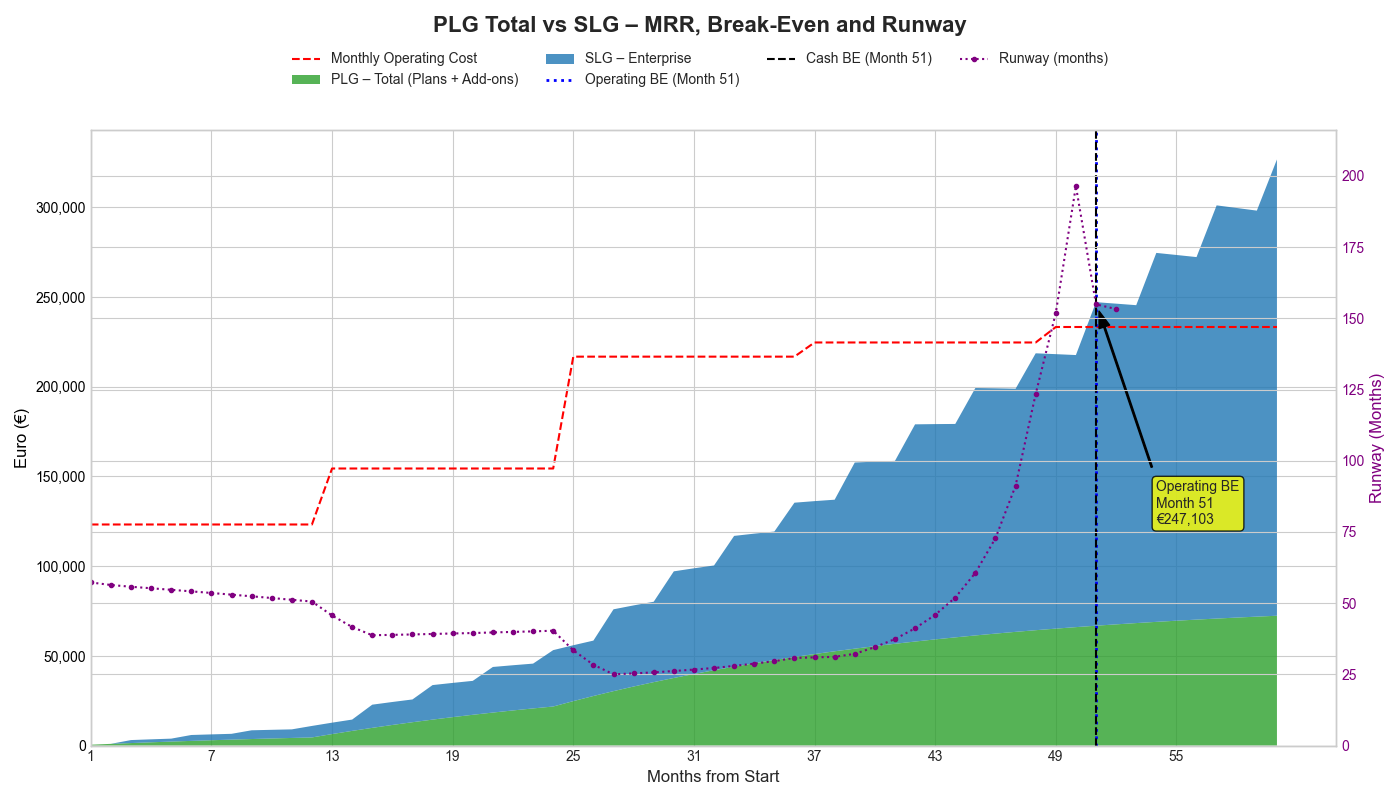
\includegraphics[width=\textwidth]{financial_projection.png}
    \caption{盈亏平衡分析:PLG 与 SLG 的 MRR、月度成本和跑道。}
    \label{fig:break_even_analysis}
\end{figure} 
\subsection{Break-even Analysis: Chart Interpretation}

\paragraph{Legend (quick read)}
\begin{itemize}
  \item \textbf{Green (PLG -- Plans + Add-ons):} 自助式经常性收入。
  \item \textbf{Blue (SLG -- Enterprise):} 企业经常性收入;以季度``阶梯''增长,因为年度合同在季度间平滑分摊。
  \item \textbf{Red dashed:} 月度运营成本(含审慎性上调),以年度阶梯上升。
  \item \textbf{Purple dotted:} 跑道(以月计),计算为现金除以3个月移动平均烧钱。
  \item \textbf{Vertical lines:} 运营盈亏平衡(蓝色,第~51 个月)和现金盈亏平衡(黑色,第~51 个月)。
\end{itemize}

在前 3 年中,图表显示了一个稳健且耐心的增长过程。绿色的 PLG 区域稳步上升,因为每月注册量在流失后复利增长,且附加组件带来增量 MRR。蓝色的 SLG 区域在企业合同签订时以明显的季度阶梯上升。成本以块状方式移动:每到新的一年都会增加计划的产能(团队、基础设施、G\&A 并包含上调),因此红线跳升后在下一次跃升前保持平稳。

这些动态与年终数据一致。到第~1 年末,成本为 \textbf{€123{,}212}/月,而经常性 MRR 为 \textbf{€10{,}948}/月(亏损 \textbf{€112{,}149}/月,现金 \textbf{€5{,}740{,}147},跑道 \textbf{50.6} 个月)。到第~2 年末:\textbf{€154{,}413} 对 \textbf{€53{,}194}(亏损 \textbf{€100{,}855}/月),现金 \textbf{€4{,}282{,}549},跑道 \textbf{40.3} 个月。到第~3 年末:\textbf{€216{,}746} 对 \textbf{€135{,}360}(亏损 \textbf{€80{,}631}/月),现金 \textbf{€2{,}239{,}361},跑道 \textbf{30.8} 个月。收入曲线明显缩小了与成本的差距,同时现金保持受控:\textbf{观察到的最小跑道为 25.0 个月},且\textbf{最高月度烧钱} 为 \textbf{€160{,}442}。

在第~4 年,差距显著缩小。较大的 SLG 阶梯使蓝色区域扩展更快,堆栈(PLG+SLG)几乎达到成本线。年末:成本为 \textbf{€224{,}646}/月,而经常性 MRR 为 \textbf{€218{,}614}/月(总收入 \textbf{€219{,}615}/月),接近收支平衡,亏损仅 \textbf{€5{,}031}/月,现金为 \textbf{€2{,}239{,}361}。由于移动平均烧钱接近零,紫色跑道线开始急剧上升。

盈亏平衡出现在 \textbf{第 51 个月}。在那时,\textbf{经常性 MRR 为 €247{,}103},而成本为 \textbf{€233{,}271}(运营盈亏平衡),且\textbf{总收入 €248{,}159} 超过成本(现金盈亏平衡)。为达到这一点,模型总共\textbf{烧掉 €4{,}939{,}370},最小现金为\textbf{€2{,}234{,}573},这也代表了\textbf{盈亏平衡时的储备(占本轮的 30.9\%)}。到第~5 年末,经常性 MRR 达到 \textbf{€326{,}645}/月($\approx$ \textbf{€3.92M ARR}),月利润为 \textbf{€94{,}565},现金为 \textbf{€2{,}673{,}539},跑道实际上变为无限。

% ----- End of translated content from: part_15.tex -----

% ----- Start of translated content from: part_16.tex -----

\paragraph{要点}
图表说明了三件事:
\begin{enumerate}
\item \emph{谁推动什么} PLG 构建基础,SLG 弥合差距
\item \emph{成本为何跳升} 有意的容量步骤并伴随审慎上调
\item \emph{现金如何受保护} 资金跑道从未崩塌(最短 25.0 个月)并随着收入堆栈超过成本而加速,正如报表指标所示。
\end{enumerate}

\begin{table}[H]
\centering
\caption{财务预测汇总(年末)}
\label{tab:financial_summary}
\resizebox{\textwidth}{!}{
\begin{tabular}{lrrrrrrr}
\toprule
\textbf{年末} & \textbf{每月成本(€)} & \textbf{经常性 MRR(€)} & \textbf{商店收入(€)} & \textbf{总收入(€)} & \textbf{每月盈亏(€)} & \textbf{现金余额(€)} & \textbf{现金跑道(月)} \\
\midrule
Year 1 & 123,212 & 10,948 & 116 & 11,064 & -112,149 & 5,740,147 & 50.6 \\
Year 2 & 154,413 & 53,194 & 364 & 53,558 & -100,855 & 4,282,549 & 40.3 \\
Year 3 & 216,746 & 135,360 & 755 & 136,115 & -80,631 & 2,823,198 & 30.8 \\
Year 4 & 224,646 & 218,614 & 1,001 & 219,615 & -5,031 & 2,239,361 & 123.5 \\
Year 5 & 233,271 & 326,645 & 1,191 & 327,836 & 94,565 & 2,673,539 & Profitable \\
\bottomrule
\end{tabular}
}
\end{table}

\begin{table}[H]
\centering
\caption{关键财务指标}
\label{tab:financial_metrics}
\resizebox{\textwidth}{!}{%
\begin{tabular}{ll}
\toprule
\textbf{指标} & \textbf{数值} \\
\midrule
运营收支平衡 & Month 51 (Year 5): Recurring MRR €247,103 $\geq$ Costs €233,271 \\
总体收支平衡 & Month 51 (Year 5): Total Revenue €248,159 $\geq$ Costs €233,271 \\
达到现金平衡前的资本消耗 & €4,939,370 \\
每月最高资本消耗 & €160,422 \\
期间最低现金 & €2,210,630 (30.9\% of round) \\
最低跑道(3个月移动平均) & 25.0 months \\
\bottomrule
\end{tabular}
}
\end{table}

\newpage
\section{为什么 CNY 59{,}829{,}055 是合适的金额}

我们请求 \textbf{CNY 59{,}829{,}055} ($\approx€7.15\text{M}$),因为这正是模型在我们的\emph{保守}情景下显示出的资本量,能够在不强制增长且保留实质安全边际的情况下,将公司带到 \textbf{第 51 个月的运营和现金收支平衡}。仿真结果明确:\textbf{达到现金平衡的累计烧钱 = €4{,}939{,}370},\textbf{平衡时手头现金 = €2{,}210{,}630}(即本轮的\textbf{30.9\%}),\textbf{路径中的最短跑道 = 25.0 个月}(3 个月移动平均),以及\textbf{每月峰值烧钱 = €160{,}422}。我们所要求的数额是模型显示的达到收支平衡所\emph{必要且充分}的资金,并包含结构性的应急缓冲。

该计划被设计为有弹性的:成本并非“极简”,而是按类别\textbf{审慎上调}(基础设施、G\&A、PLG、SLG、R\&D、管理层),以覆盖常被低估的经常性项目(企业支持、审计、法律、招聘、监控)。此外,模型引入了\textbf{自动护栏}:若跑道低于 12 个月,\textbf{下一月可自由支配开支削减 10\%};低于 9 个月时,\textbf{付费 PLG 获客被抑制}(乘数 0.7)。这些是模型中编码的操作规则,不是承诺。实际上,下行风险由会自动触发的机制保护。

在收入方面,我们清晰地区分了\textbf{PLG}(方案 + 附加项)和\textbf{SLG}(企业)。这不是形式上的区分:它使我们能够逐月观察各项支出杠杆的回报,并在无需意识形态干扰的情况下进行再平衡。凭借这种组合和当前定价,\textbf{运营收支平衡}在\textbf{第 51 个月}到达,其时\textbf{经常性 MRR 为 €247{,}103},而\textbf{每月成本为 €233{,}271};同月,\textbf{现金收支平衡}也实现,因为\textbf{总收入(€248{,}159)}超过成本。到第 $\sim 5$ 年末,经常性 MRR 达到 \textbf{€326{,}645}($\approx$ \textbf{€3.92M ARR})。在资本效率方面,\textbf{隐含烧钱倍数}(达到平衡的累计烧钱 $\div$ 平衡时的 ARR)约为 \textbf{1.66x},这与保守的产品+市场建构一致,且成本已被可信地上调。

那么,为什么是\emph{这个}金额,而不是更少?如果资本更少,模型会更频繁触发护栏,造成运营上的断停(削减/冷却期),延长时间线并在关键连续性时刻提高机会成本。为什么不是更多?因为超出该阈值的资本并不能解决瓶颈——瓶颈在于\textbf{渠道吸收能力}和企业交付的自然节奏;今天额外的现金只会增加摊薄,而无法相对于模型改善结果。

\textbf{资金用途}仍锚定于仿真中的各类及其上调:产品/研发(硬化、可观测性、安全)、基础设施 \& 企业支持、SLG(客户、解决方案/POC)、PLG(内容/SDK/社区)、合作伙伴赋能、G\&A \& 合规、管理层。我们并未开辟新的支出线:我们是在为模型已逐月衡量的事项提供资金。

最后,\textbf{风险轮廓}是可读的。最短跑道不低于\textbf{25.0 个月},护栏在需要时限制现金侵蚀,且收支平衡时的\textbf{30.9\%} 缓冲为采购延迟、基础设施/合规开支波动或外汇变动提供了余地。与此同时,PLG/SLG 的分离使得即便事后评估也能清楚显示资本配置是遵循已实现回报而非一刀切的计划。

\textbf{简言之:} \textbf{CNY 59{,}829{,}055} 充分资助了通往保守路径下收支平衡的过程,具有足够的缓冲和自动化的成本纪律。这是一个比例合理、可辩护且——最重要的——\textbf{可复现}的请求:投资方可以逐月核实模型指标是否受控以及现金是否沿预期轨迹运行。

\subsection{战略缓冲理由:在 AI 编排前沿航行}
收支平衡时的 30.9\% 资本储备(€2.21M)代表了一项有意的战略配置,用于在 AI 编排市场前所未有的变动速度中航行。与传统 SaaS 领域中产品市场契合遵循可预测模式不同,AI 基础设施领域每 3-6 个月就发生根本性变化——从新的 LLM 架构到像 MCP 这样的新兴编排标准。该缓冲使 IntellyHub 能够在不危及跑道的情况下执行快速战略转向:无论是适应自治代理能力的突破、整合规划时不存在的颠覆性模型,还是根据真实市场反应在 PLG 与 SLG 之间转移焦点。成功的 AI 基础设施公司的历史先例(Weights \& Biases、Hugging Face)表明,赢者通常在实现可持续增长前需要进行 2-3 次重大转向——每次消耗可用资本的 15-20\%。我们的储备确保我们至少能在保持 12+ 个月运营跑道的同时执行一次重大战略调整,将本可能成为生存威胁的情形转化为竞争优势。这并非过剩资本;它是在一个唯一确定性是剧烈变化的市场中,为快速于竞争对手完成转向而准备的经过计算的可选性保险——当竞争者为紧急融资慌乱时,快速转向的能力成为市场领先与被淘汰之间的决定性因素。

\newpage
\section{Go-to-Market 战略}
% 如何接触到你的客户?

IntellyHub 的 Go-to-Market(GTM)战略基于一种融合两大增长引擎的混合模型:
\begin{enumerate}
    \item \textbf{Product-Led Growth (PLG) for SaaS:} 我们利用产品优势、免费层和自动化商店,以可扩展的自下而上方式吸引、激活并转化用户。
    \item \textbf{Sales-Led Growth (SLG) for On-Premise \& Enterprise:} 我们采用有针对性的咨询式销售方法,争取具有复杂安全与治理需求的大客户。
\end{enumerate}
这两大引擎被设计为相互增强:PLG 动作的成功为销售团队产生线索和品牌认知。

% ----- End of translated content from: part_16.tex -----

% ----- Start of translated content from: part_17.tex -----

\subsection{战略目标(3 年期)}
\begin{itemize}
    \item \textbf{定位:} 成为为现代技术团队协调复杂自动化和 AI 工作流的领先平台。
    \item \textbf{采纳:} 实现活跃用户的临界规模,并围绕插件生态系统与自动化商店形成充满活力的社区。
    \item \textbf{营收:} 建立可持续的商业模式,实现显著的年经常性收入(ARR),由 SaaS 订阅和企业本地部署合同共同驱动。
\end{itemize}

% --- YEAR 1 ---
\subsection{第一年:基础 \& 市场验证}
\textbf{主要关注:} 赢得早期采用者,验证产品-市场契合度,并获取首批关键参考客户(包括 SaaS 和本地部署)。在此阶段,许多活动是手动的且“不可规模化”。

\newpage
\begin{table}[H]
\centering
\resizebox{\textwidth}{!}{
\begin{tabularx}{\textwidth}{L L L} 
\toprule
\textbf{关键渠道} & \textbf{具体行动} & \textbf{成功 KPI} \\

\midrule
\textbf{产品驱动增长(PLG)} & 
\textbf{利基发布:} 在 Product Hunt、Hacker News 和相关技术子版块(例如 r/devops、r/kubernetes)上展示 IntellyHub。\newline\newline
\textbf{自动化商店:} 在商店中填充 20-30 个高质量的官方模板,解决真实且痛点明显的问题。
&
\textbf{激活率:} >25\%(用户在 7 天内运行其第一个自动化)。\newline\newline
\textbf{1 个月留存:} >15\%(用户在 4 周后回访)。
\\
\addlinespace

\textbf{技术内容营销} & 
\textbf{博客 \& 教程:} 每月发布 2-4 篇深入的技术文章,展示如何使用 IntellyHub 解决具体问题。\newline\newline
\textbf{视频内容:} 制作简练的视频教程。
&
\textbf{合格流量:} 来自自然和推荐渠道的网站访问量。\newline\newline
\textbf{访客到注册率:} >2\%.
\\
\addlinespace

\textbf{社区建设} &
\textbf{Discord/Slack 频道:} 为早期用户建立一个中心枢纽。\newline\newline
\textbf{由创始人主导的支持:} 创始人亲自回答每一个问题和反馈请求,以建立牢固的关系。
&
\textbf{社区参与度:} 每周活跃成员数、用户间互助互动。\newline\newline
\textbf{定性反馈:} 每月至少进行 5 次深入用户访谈。
\\
\addlinespace

\textbf{创始人主导销售(本地部署)} &
\textbf{利用网络:} 创始人亲自管理首批与其自身网络目标公司之间的 3-5 个销售流程。\newline\newline
\textbf{概念验证(POC):} 专注于少数高价值 POC 的成功。
&
\textbf{启动的 POC:} 全年 3-5 个。\newline\newline
\textbf{签署的本地部署合同:} 1-2 个关键参考客户。
\\
\bottomrule
\end{tabularx}
}
\end{table}


% --- YEAR 2 ---
\newpage
\subsection{第二年:扩张 \& 构建可复制的增长引擎}
\textbf{主要关注:} 将初期价值转化为可规模化、可复制的流程。优化第一年有效的内容,并建立商业团队的基础。

\begin{table}[H]
\small
\centering
\resizebox{\textwidth}{!}{
\begin{tabularx}{\textwidth}{L L L}
\toprule
\textbf{关键渠道} & \textbf{具体行动} & \textbf{成功 KPI} \\
\midrule
\textbf{PLG 优化} &

\textbf{漏斗分析:} 使用分析工具识别并消除从注册到付费转化过程中用户旅程中的摩擦点。
\textbf{引导式入职:} 实施应用内入职体验,带领新用户达到他们的“ Aha! ”时刻。
&

\textbf{免费到付费转化率:} >3\%.

% ----- End of translated content from: part_17.tex -----

% ----- Start of translated content from: part_18.tex -----

\textbf{MRR 增长率:} 持续逐月增长。
\\
\addlinespace
\textbf{生态系统合作伙伴} &

\textbf{战略集成:} 积极为2-3个拥有相似用户群的互补技术平台开发插件。
\textbf{联合营销:} 与合作伙伴发起联合营销活动(网络研讨会、博客文章)。
&

\textbf{来自合作伙伴的潜在客户。}
\textbf{合作伙伴插件的下载量。}
\\
\addlinespace
\textbf{初始销售团队} &

\textbf{首批招聘:} 另外招聘一名客户经理以处理进站线索并开始有针对性的外呼拓展。
\textbf{销售手册:} 根据创始人主导销售阶段的经验教训使销售流程制度化。
&

\textbf{每月合格演示次数。}
\textbf{平均销售周期时长(本地部署)。}
\\
\bottomrule
\end{tabularx}
}
\end{table}

\newpage
% --- 第三年 ---
\subsection{第三年:规模化 \& 细分市场领导}
\textbf{主要关注点:} 加速增长,主导技术团队细分市场,并将 IntellyHub 建立为 AI 编排市场的思想领袖。

\begin{table}[H]
\centering
\resizebox{\textwidth}{!}{
\begin{tabularx}{\textwidth}{L L L}
\toprule
\textbf{关键渠道} & \textbf{具体行动} & \textbf{成功关键绩效指标} \\
\midrule
\textbf{销售可扩展性} &

\textbf{团队扩展:} 扩大销售团队以覆盖不同的地理区域或行业垂直领域。
\textbf{间接渠道:} 开始探索与系统集成商和经销商的合作。
&

\textbf{年度经常性收入(ARR)增长。}
\textbf{客户获取成本(CAC)及 LTV/CAC 比率。}
\\
\addlinespace
\textbf{品牌营销} &

\textbf{思想领导力:} 基于平台聚合数据发布行业报告。
\textbf{赞助:} 赞助 DevOps 与 AI 领域的关键会议和播客。
&

\textbf{行业媒体报道次数。}
\textbf{直接 \& 品牌流量的增长。}
\\
\addlinespace
\textbf{网络效应} &

\textbf{开放商店:} 向外部贡献者和合作伙伴开放 Automation Store 与插件市场。
\textbf{开发者计划:} 启动正式的开发者关系(DevRel)计划。
&

\textbf{社区创建插件/模板的数量。}
\textbf{净收入留存率(NRR):} >110\%.
\\
\bottomrule
\end{tabularx}
}
\end{table}

\clearpage
\section{运营计划}
% 公司日常运作方式。
\subsection{介绍}
本文件概述了执行 IntellyHub 开发与市场进入战略的运营计划。该计划与产品开发路线图的各阶段保持一致,并描述了公司各职能领域的关键活动。

% --- 第1阶段 ---

% ----- End of translated content from: part_18.tex -----

% ----- Start of translated content from: part_19.tex -----

\subsection{阶段1:基础与验证(第1-2季度)}
\textbf{战略目标:} 将原型转变为稳定且安全的 MVP,获取首批早期采用者,并通过一个针对性的合作伙伴计划\textbf{验证核心产品与定价模型假设。}

\subsubsection{产品开发 \& 工程}
\begin{itemize}[leftmargin=*]
    \item \textbf{Q1:}
    \begin{itemize}
        \item \textbf{Stabilization:} 完成测试套件(单元测试、集成测试),以确保核心引擎的可靠性。
        \item \textbf{Plugin:} 完成并记录内部系统,以支持标准化插件开发。
        \item \textbf{UI/UX:} 优化混合型 IDE 界面,解决任何同步问题并提升用户体验。
        \item \textbf{On-Premise:} 为企业客户开发并测试平台的本地部署版本。
    \end{itemize}
    \item \textbf{Q2:}
    \begin{itemize}
        \item \textbf{Authentication:} 实施健壮的用户管理与认证系统。
        \item \textbf{Onboarding:} 为新用户开发一个引导式入门向导。
        \item \textbf{Store (v1):} 为首个版本的自动化商店(只读)创建 API 与 UI。
    \end{itemize}
\end{itemize}

\subsubsection{Go-to-Market (Marketing \& Sales)}
\begin{itemize}[leftmargin=*]
    \item \textbf{Q1-Q2:}
    \begin{itemize}
        \item \textbf{Vertical Strategy:} 在一个\textit{初始垂直细分领域}内定义详细的理想客户画像(ICP)(例如:生物技术/科学研究,基于 Esplorado 的用户案例)。
        \item \textbf{(New) Design Partner Program:} 为目标垂直中的 3-5 家精选公司启动一个独家计划。提供提前访问和直接支持,以换取持续反馈和潜在的初步合同。
    \end{itemize}
    \item \textbf{Q3-Q4:}
    \begin{itemize}
        \item \textbf{Niche Launch:} 在 Product Hunt、Hacker News 及相关渠道执行上线,传播重点聚焦于所选垂直领域。
        \item \textbf{Feedback Collection:} 从免费层用户以及优先级为设计合作伙伴的用户处收集结构化反馈。
    \end{itemize}
\end{itemize}

\subsubsection{Community \& Ecosystem Management}
\begin{itemize}[leftmargin=*]
    \item \textbf{Q1-Q2:}
    \begin{itemize}
        \item \textbf{Targeted Plugin Development:} 开发并记录首批“官方”插件,\textit{优先考虑与目标垂直最相关的那些}。
    \end{itemize}
    \item \textbf{Q3-Q4:}
    \begin{itemize}
        \item \textbf{Community Creation:} 启动官方 Discord/Slack 服务器。
        \item \textbf{Engagement:} 创始人和开发团队将积极参与,回答问题并营造友好的氛围。
    \end{itemize}
\end{itemize}

\subsubsection{General \& Corporate Operations}
\begin{itemize}[leftmargin=*]
    \item \textbf{Q1-Q2:}
    \begin{itemize}
        \item \textbf{Legal and Administrative Setup:} 确定公司架构,开设银行账户。
        \item \textbf{(New) Partner Contracting:} 为“设计合作伙伴计划”准备相关协议。
    \end{itemize}
    \item \textbf{Q3-Q4:}
    \begin{itemize}
        \item \textbf{Terms of Service Definition:} 为免费层上线撰写并发布服务条款与隐私政策。
    \end{itemize}
\end{itemize}

\clearpage

% --- PHASE 2 ---
\subsection{阶段2:扩展与增长(第3-4季度)}
\textbf{战略目标:} 在第一阶段验证的数据基础上,扩大用户获取,扩展生态系统,并实现面向企业的变现所需功能。

\subsubsection{产品开发 \& 工程}
\begin{itemize}[leftmargin=*]
    \item \textbf{Q5-Q6:}
    \begin{itemize}
        \item \textbf{Security:} 为凭证实现一个秘密管理系统。
        \item \textbf{Versioning:} 为自动化添加历史记录和回滚功能。
    \end{itemize}
    \item \textbf{Q7-Q8:}
    \begin{itemize}
        \item \textbf{Observability:} 开发首个用于流程性能指标的数据平台版本。
        \item \textbf{Improve Dashboards:} 创建用于可视化流程的用户界面。
        \item \textbf{Proactive AI:} 基于流程性能数据实现基础的“自动修复”功能。
    \end{itemize}
\end{itemize}

% ----- End of translated content from: part_19.tex -----

% ----- Start of translated content from: part_20.tex -----

\subsubsection{上市策略 (Marketing \& Sales)}
\begin{itemize}[leftmargin=*]
    \item \textbf{Q5-Q6:}
    \begin{itemize}
        \item \textbf{垂直内容营销:} 扩大内容生产规模(基于 Design Partners 的案例研究、文章),聚焦所选垂直领域。
        \item \textbf{招聘:} 开始首位开发者倡导者 (Developer Advocate) 的招聘流程。
    \end{itemize}
    \item \textbf{Q7-Q8:}
    \begin{itemize}
        \item \textbf{付费方案上线:} 确定定价(已与 Design Partners 验证),并正式推出 Pro 和 Enterprise 方案。
        \item \textbf{销售手册 (v1):} 开始记录企业客户的销售流程。
    \end{itemize}
\end{itemize}

\clearpage

% --- PHASE 3 ---
\subsection{Phase 3: Leadership and Innovation (Quarters 5-6)}
\textbf{Strategic Objective:} 建立市场领导地位,通过社区创造网络效应,并 **利用数据构建不可逾越的竞争优势。**

\subsubsection{Product Development \& Engineering}
\begin{itemize}[leftmargin=*]
    \item \textbf{Q9-Q10:}
    \begin{itemize}
        \item \textbf{Store Opening:} 开放 Store,允许社区提交内容。
        \item \textbf{Moderation:} 实现用于审查和验证外部贡献的内部工具。
    \end{itemize}
    \item \textbf{Q11-Q12:}
    \begin{itemize}
        \item \textbf{(Revised) Data Platform \& Observability:} 开发用于收集和聚合流性能指标的系统,战略目标是 \textbf{构建 "数据护城河"}。
        \item \textbf{Analytics Dashboard:} 创建用于可视化分析的用户界面。
        \item \textbf{Proactive AI:} 改进“自动修复”(auto-healing)和主动优化功能,\textbf{基于聚合的平台数据进行训练}。
    \end{itemize}
\end{itemize}

\subsubsection{Go-to-Market (Marketing \& Sales)}
\begin{itemize}[leftmargin=*]
    \item \textbf{Q9-Q10:}
    \begin{itemize}
        \item \textbf{Sales Team Scaling:} 招聘额外的客户经理(Account Executives),以覆盖特定市场或行业垂直领域。
        \item \textbf{Thought Leadership:} 开始发布基于平台使用数据的报告和分析。
    \end{itemize}
    \item \textbf{Q11-Q12:}
    \begin{itemize}
        \item \textbf{Brand Marketing:} 增加在品牌知名度活动(赞助、活动)上的投入。
    \end{itemize}
\end{itemize}

\newpage
\section{Risk Analysis}
\subsection{Market Risks}
\textit{与市场、竞争和客户采用相关的风险。}

\begin{table}[H]
\centering
\begin{tabularx}{\textwidth}{@{}lL@{}}
\toprule
\textbf{Risk} & \textbf{Description} \\
\midrule
\textbf{来自“现状”的竞争} & 我们最大的竞争对手不是另一个平台,而是开发者使用自定义 Python 脚本的惯性。他们的熟悉程度和被认为的零初始成本构成了一个显著的障碍。 \\
\addlinespace
\textbf{企业采纳周期缓慢} & 本地部署和企业销售模型对高价值合同至关重要,但其特点是长销售周期(6-12+ 个月)和复杂的概念验证(POC)阶段。首批关键企业交易的延迟可能会显著影响收入预测。 \\
\addlinespace
\textbf{AI 技术转变} & 我们的 AI 目前定位为“copilot”。竞争对手若在技术上迅速跃进,推出一个“足够好”的真正自治 AI 代理,可能会使我们更受控、更结构化的方法显得不够创新。 \\
\bottomrule
\end{tabularx}
\end{table}

\newpage
\subsection{Operational Risks}
\textit{与技术、人员和执行相关的风险。}

\begin{table}[H]
\centering
\begin{tabularx}{\textwidth}{@{}lL@{}}
\toprule
\textbf{Risk} & \textbf{Description} \\
\midrule
\textbf{团队执行 \& 关键人物风险} & 该计划依赖于招聘少数高度专业化的人才。项目的成功在很大程度上取决于该核心团队在产品、基础设施和销售方面的执行能力。关键成员的离职可能导致重大延误。 \\

% ----- End of translated content from: part_20.tex -----

% ----- Start of translated content from: part_21.tex -----

\addlinespace
\textbf{技术复杂性} & 技术栈(Kubernetes、多步骤 AI 流水线、混合 IDE)功能强大,但维护和演进也非常复杂。该复杂系统中的错误、安全漏洞或性能瓶颈可能难以定位且修复代价高昂。 \\
\addlinespace
\textbf{混合技术风险(IDE/YAML 同步)} & 在复杂的可视化 IDE 与文本化的 YAML 表示之间保持完美、实时、双向同步在技术上要求很高。这可能成为微妙且难以调试的错误来源,从而影响用户信任。 \\
\addlinespace
\textbf{生态系统质量控制} & 自动化商店和插件市场的价值是一把双刃剑。低质量、不安全或维护不善的社区贡献可能会损害用户信任和平台声誉。 \\
\bottomrule
\end{tabularx}
\end{table}

\newpage
\subsection{财务风险}
\textit{与现金流、融资和财务可持续性相关的风险。}

\begin{table}[H]
\centering
\begin{tabularx}{\textwidth}{@{}lL@{}}
\toprule
\textbf{风险} & \textbf{描述} \\
\midrule
\textbf{高额的初期现金消耗} & 进取的招聘计划在产生显著收入之前会导致高额的月度运营成本。这给实现产品—市场契合并快速产生收入带来巨大压力。 \\
\addlinespace
\textbf{对融资的依赖} & 该商业模式并非为短期盈利而设计。未能达到投资者预期的增长关键绩效指标将构成生存性威胁。 \\
\addlinespace
\textbf{定价模型验证} & 所提出的价值度量(执行次数、活跃自动化)在逻辑上有道理,但未经过验证。不正确的定价模型可能导致客户摩擦(如果太贵)或流失大量潜在收入(如果太便宜)。 \\
\bottomrule
\end{tabularx}
\end{table}

\newpage
\subsection{缓解策略}
\textit{用以应对并降低已识别风险的具体行动。}

\begin{table}[H]
\centering
\begin{tabularx}{\textwidth}{@{}lL@{}}
\toprule
\textbf{风险类别} & \textbf{缓解策略} \\
\midrule
\textbf{市场风险} & 
\textbf{定位 \& 教育:} 将营销重点放在消除管理大量脚本所带来的长期混乱上,而不是替代单个脚本。使用像 "Esplorado" 这样的案例研究来提供不可否认的价值证明。 \newline\newline
\textbf{混合 GTM:} 同时开展 PLG(SaaS)和 SLG(本地部署)两条路线。利用来自 PLG 端更快的反馈循环来改进产品和信息传达,从而适应更慢的企业销售周期。 \newline\newline
\textbf{战略性 AI 路线图:} 将当前的 AI 定位为面向生产环境的务实、安全且可靠的选择。将路线图表述为在我们已有的稳固基础上,逐步演进到更具自主能力的方向。 \\
\addlinespace
\textbf{运营风险} & 
\textbf{文档 \& 交叉培训:} 从第一天起大量投入内部文档建设。实施知识共享文化和结对编程,以减少对单一个人员的依赖。 \newline\newline
\textbf{投资可观测性 \& 测试:} 投入资源构建健全的自动化测试套件,并尽早集成应用性能监控(APM)工具,以主动识别和解决问题。测试套件应专门覆盖 IDE/YAML 同步逻辑。 \newline\newline
\textbf{策划的生态系统:} 初期商店仅展示“官方”和“认证合作伙伴”插件。为未来所有社区提交实现明确且严格的审查流程,包括自动化安全扫描和质量检查。 \\
\addlinespace
\textbf{财务风险} & 
\textbf{基于里程碑的支出:} 将重大支出增加(尤其是市场和销售人员的招聘)与特定的、预先定义的里程碑绑定(例如,达到前 10 名付费客户,达到某一留存率)。 \newline\newline
\textbf{持续的投资者关系:} 与现有和潜在未来投资者保持透明且定期的沟通渠道,分享关键绩效指标的进展,以建立信心并简化下一轮融资。 \newline\newline
\textbf{定价迭代:} 以简单且灵活的定价模型上线。直接与早期客户互动,了解他们所获得的价值,并准备根据他们的反馈和使用数据迭代定价结构。 \\
\bottomrule
\end{tabularx}
\end{table}

% \newpage
% \subsection{产品截图}
% 屏幕截图、模型或产品图表。

\newpage
% 在此添加引用、研究或文章。
\begin{thebibliography}{99}
    \bibitem{AIMarket}
    Market.us, \textit{自动化机器学习市场报告}, 可在:\url{https://market.us/report/automated-machine-learning-market/} 获取,2025年3月。
    
    \bibitem{MLOpsMarket}
    MarketReserchFuture.com, \textit{MLOps 市场研究报告:按组件(服务、平台)、按部署模式(本地部署、云)、按组织规模(大型企业、中小企业)、按行业(BFSI、零售与电子商务、政府与国防、医疗与生命科学、制造业及其他)和按地区(北美、欧洲、亚太及世界其他地区)划分——市场预测至 2034 年。}, 可在:\url{https://www.marketresearchfuture.com/reports/mlops-market-18849} 获取,Agoust~2025。
    
    \bibitem{AIOrch}
    Market.us, \textit{AI 编排平台市场报告 (2024--2034 预测)}, 2025年2月。  
    可在:\url{https://market.us/report/ai-orchestration-platform-market/} 获取。

    \bibitem{GartnerAgentic}
    Reuters(转述 Gartner),\textit{超过 40\% 的具代理性的 AI 项目将在 2027 年前被放弃……到 2028 年,33\% 的企业软件将包含具代理性的 AI,且 15\% 的决策将由系统自主作出,} 2025年6月25日。  
    可在:\url{https://www.reuters.com/business/over-40-agentic-ai-projects-will-be-scrapped-by-2027-gartner-says-2025-06-25/} 获取。

    \bibitem{MLOpsMM}
    MarketsandMarkets Research, \textit{MLOps 市场规模预计到 2027 年将超过 US\$5.9 Billion,复合年增长率为 41.0\%}, 2023年4月21日。  

    可在以下地址获取:\url{https://www.globenewswire.com/news-release/2023/04/21/2652028/0/en/MLOps-Market-Size-is-Anticipated-to-Cross-US-5-9-billion-by-2027-growing-at-a-CAGR-of-41-0-Report-by-MarketsandMarkets.html}.

    \bibitem{ModelOpsGV}
    Grand View Research, \textit{ModelOps 市场报告}, 2025 年版。  
    可在以下地址获取:\url{https://www.grandviewresearch.com/industry-analysis/modelops-market-report}.

    \bibitem{AIMLMarket}
    Market.us, \textit{自动化机器学习市场报告(2024--2034 预测)}, 2025年3月。  
    可在以下地址获取:\url{https://market.us/report/automated-machine-learning-market/}.

    \bibitem{MLOpsMRF}
    MarketResearchFuture, \textit{MLOps 市场研究报告(2024--2034 预测)}, 2025年8月。  
    可在以下地址获取:\url{https://www.marketresearchfuture.com/reports/mlops-market-18849}.

    \bibitem{deloitte2020}
    Deloitte, \textit{基于智能边缘的自动化:为超级赋能企业开辟的新前沿}, 2020。 可在以下地址获取:\url{https://www2.deloitte.com/us/en/insights/topics/talent/intelligent-automation-2020-survey-results.html}

    \bibitem{grandviewRPA}
    Grand View Research, \textit{机器人流程自动化 (RPA) 市场规模、份额 \& 趋势分析报告}, 2024。可在以下地址获取:\url{https://www.grandviewresearch.com/industry-analysis/robotic-process-automation-rpa-market}

    \bibitem{mckinseyAI2023}
    McKinsey \& Company, \textit{2023 年 AI 现状:生成式 AI 的爆发之年}, 2023年8月1日。可在以下地址获取:\url{https://www.mckinsey.com/capabilities/quantumblack/our-insights/the-state-of-ai-in-2023-generative-ais-breakout-year}


    \bibitem{langchainGitHub}
    LangChain GitHub 仓库。可在以下地址获取:\url{https://github.com/langchain-ai/langchain}

    \bibitem{gartnerAIBarriers}
    Gartner, \textit{AI 采用的两大障碍}, 2021年11月2日。可在以下地址获取:\url{https://www.gartner.com/en/articles/2-barriers-to-ai-adoption}

    \bibitem{euAIAct}
    European Commission, \textit{关于人工智能的监管框架提案}. 可在以下地址获取:\url{https://digital-strategy.ec.europa.eu/en/policies/regulatory-framework-ai}
    
    \bibitem{AIOrch}
    Market.us, \textit{AI 协同平台市场报告(2024--2034 预测)}, 2025年2月。可在以下地址获取:\url{https://market.us/report/ai-orchestration-platform-market/}.

    \bibitem{zapierApps}
    Zapier, \textit{探索 6,000+ 个应用}. 可在以下地址获取:\url{https://zapier.com/apps}

    \bibitem{g2ZapierReviews}
    G2, \textit{Zapier 评价}. 可在以下地址获取:\url{https://www.g2.com/products/zapier/reviews}

    \bibitem{zapierPricing}
    Zapier, \textit{Zapier 定价方案}. 可在以下地址获取:\url{https://zapier.com/pricing}


    \bibitem{zapierOpenAI}
    Zapier, \textit{OpenAI 集成}. 可在以下地址获取:\url{https://zapier.com/apps/openai/integrations}

    \bibitem{g2MakeVsZapier}
    G2, \textit{Make 与 Zapier 的比较}. 可在以下地址获取:\url{https://www.g2.com/compare/make-vs-zapier}


    \bibitem{autogenGitHub}
    Microsoft, \textit{AutoGen GitHub 仓库}. 可在以下地址获取:\url{https://github.com/microsoft/autogen}

    \bibitem{crewaiGitHub}
    Joao Moura, \textit{CrewAI GitHub 仓库}. 可在以下地址获取:\url{https://github.com/joaomdmoura/crewAI}

    \bibitem{langchainValuation}
    TechCrunch, \textit{AI 基础设施初创公司 LangChain 据称筹资 $100M,估值 $1.1B}, 2025年7月9日。可在以下地址获取:\url{https://siliconangle.com/2025/07/09/ai-infrastructure-startup-langchain-reportedly-raises-100m-1-1b-valuation/#:~:text=Artificial%20intelligence%20infrastructure%2C%20developer%20tools,on%20a%20%241.1%20billion%20valuation.}

    \bibitem{langchainIntegrations}
    LangChain Documentation, \textit{LangChain 集成}. 可在以下地址获取:\url{https://python.langchain.com/docs/integrations/providers/}

    \bibitem{langchainCritique}
    Medium, \textit{LangChain 的挑战 \& 批评}, 2025年3月3日。可在以下地址获取:\url{https://shashankguda.medium.com/challenges-criticisms-of-langchain-b26afcef94e7}

    \bibitem{mrfRPA}
    Market Research Future, \textit{机器人流程自动化 (RPA) 市场研究报告信息:按流程(决策支持、自动化解决方案与管理解决方案)、按运营(基于规则与基于知识)、按行业(制造 \& 物流,以及 IT \& 电信)、按地区(北美、欧洲、亚太及世界其他地区)——行业规模、份额及 2032 年预测}. 可在以下地址获取:\url{https://www.marketresearchfuture.com/reports/robotic-process-automation-market-2209}

    \bibitem{uipathGartner}
    UiPath, \textit{Gartner 机器人流程自动化魔力象限}, 2025。可在以下地址获取:
    \url{https://www.uipath.com/resources/automation-analyst-reports/gartner-magic-quadrant-robotic-process-automation}

    \bibitem{awsSagemaker}
    Amazon AWS SageMaker, \textit{Amazon SageMaker}, 可在以下地址获取:\url{https://aws.amazon.com/sagemaker/}

    \bibitem{forresterRPAvsAI}
    Craig Le Clair, \textit{RPA 平台会继续保持相关性吗?AI 代理或许能给出答案。}, Forrester, 2024年4月25日。可在以下地址获取:\url{https://www.forrester.com/blogs/will-rpa-platforms-remain-relevant-ai-agents-may-hold-the-answer/}

% ----- End of translated content from: part_22.tex -----

% ----- Start of translated content from: part_23.tex -----

\end{thebibliography}


\end{document}

% ----- End of translated content from: part_23.tex -----

